\documentclass[a4paper]{article}
\usepackage{listings}
\usepackage{multicol}
\usepackage[utf8]{inputenc}
\usepackage{amsmath}
\usepackage{amssymb}
\usepackage{microtype}
\usepackage[maxbibnames=99]{biblatex}
\usepackage{url}\urlstyle{tt}
\input{include/asp-macros/dtel}
\input{include/asp-macros/logics}
\input{include/asp-macros/systems}


\renewcommand{\wnext}{\ensuremath{\widehat{\Next}}}

\newcommand{\eqdef}{\ensuremath{=^{def}}}

\newcommand{\equivht}{\stackrel{\normalfont\mbox{\tiny HT}}{\equiv}}
\newcommand{\equivtht}{\stackrel{\normalfont\mbox{\tiny THT}}{\equiv}}


% temporal formalities

\newcommand{\s}[1]{\ensuremath{``#1"\,}}

\newcommand{\nnf}{\ensuremath{\mathit{nnf}\,}}
\newcommand{\AFW}{\ensuremath{\mathrm{AFW}}}

\newcommand{\PV}{\ensuremath{\mathcal{P}}}
\newcommand{\Rel}[2]{\parallel\!#1\!\parallel^{#2}}

\newcommand*{\defeq}{\stackrel{\text{def}}{=}}

% \usepackage{include/comments/comments}
\usepackage{xcolor}
\usepackage{tikz}
\usepackage[framemethod=tikz]{mdframed}
\usepackage[font=footnotesize]{caption}

% For exported plots and tables
\usepackage{booktabs}
\usepackage[utf8]{inputenc}
\usepackage{pgfplots}
\DeclareUnicodeCharacter{2212}{−}
\usepgfplotslibrary{groupplots,dateplot}
\usetikzlibrary{patterns,shapes.arrows}
\pgfplotsset{compat=newest}

\usepackage{subcaption}
\usepackage[T1]{fontenc}
\usepackage[toc,page]{appendix}
\usepackage{amsmath,amsthm,amssymb}
\usepackage[inline]{enumitem}


\lstdefinelanguage{clingo}{
  keywordstyle=[1]\usefont{OT1}{cmtt}{m}{n},%
  keywordstyle=[2]\textbf,%
  keywordstyle=[3]\usefont{OT1}{cmtt}{m}{n},%\textit
  alsoletter={\#,\&},%
  keywords=[1]{not,from,import,def,if,else,return,while,break,and,or,for,in,del,and,class},%
  keywords=[2]{\#const,\#show,\#minimize,\#base,\#theory,\#count,\#external,\#program,\#script,\#end,\#heuristic,\#edge,\#project,\#show},%
  keywords=[3]{&,&dom,&sum,&diff,&show,&minimize},%
  morecomment=[l]{\#\ },%
  morecomment=[l]{\%\ },%
  commentstyle={\color{darkgray}}%
}
\lstset
{ %Formatting for code in appendix
    literate={~}{{\fontfamily{ptm}\selectfont \textasciitilde}}1,
    language=clingo,
    basicstyle=\ttfamily\footnotesize,
    numbers=left,
    stepnumber=1,
    showstringspaces=false,
    tabsize=1,
    breaklines=true,
    breakatwhitespace=false,
    frame=single,
    xleftmargin=2em
}

\usetikzlibrary{arrows,automata,positioning}

%%%%%%%%%%%%%%%%%%%%% Formats %%%%%%%%%%%%%%%%%%%%%%
\definecolor{darkgreen}{rgb}{0,0.5,0}
\definecolor{darkblue}{HTML}{00305E}
\definecolor{darkred}{rgb}{0.8,0,0}
\newtheoremstyle{exampstyle}
{7pt} % Space above
{7pt} % Space below
{} % Body font
{} % Indent amount
{\bfseries} % Theorem head font
{.} % Punctuation after theorem head
{.5em} % Space after theorem head
{\thmname{#1}\thmnumber{ #2} \thmnote{(\emph{#3})}}%                                     % Theorem head spec (can be left empty, meaning `normal')

\theoremstyle{exampstyle}
\newtheorem{definition}{Definition}
\newtheorem{theorem}{Theorem}
\newtheorem{lemma}{Lemma}
\newcounter{example}
\newenvironment{example}[1][]{\refstepcounter{example}\par\medskip
\noindent \textcolor{black!45}{\textbf{Example~\theexample. #1}}
\par\nopagebreak%
\begin{mdframed}[
   linewidth=3pt,
   linecolor=black!17,
   bottomline=false,topline=false,rightline=false,
   innerrightmargin=0pt,innertopmargin=0pt,innerbottommargin=0pt,
   innerleftmargin=1em,% Distance between vertical rule & proof content
   skipabove=.5\baselineskip
 ]}
{\end{mdframed}}

\bibliography{krr,procs}
\bibliography{local-bib}

\begin{document}


\begin{titlepage}
    \begin{center}
    
    \begin{center}
      
\includegraphics[scale=0.2]{uni-potsdam.jpg}
    \end{center}
    \vspace*{.008\textheight}
    {\scshape\LARGE \textcolor{darkblue}{University Of Potsdam}\par}
    
    \large 
    \textcolor{darkblue}{\emph{Cognitive Systems: Language, Learning and Reasoning}}
    
    \vspace{1.5cm}
    \textsc{\Large Master's Thesis}\\[0.5cm]
    
    \noindent\rule{\textwidth}{0.3mm}
    {\huge \bfseries Advanced Meta-Answer Set Programming\par}\vspace{0.4cm}
    \noindent\rule{\textwidth}{0.3mm}
     
    \vspace*{.005\textheight}
    \begin{minipage}[t]{0.4\textwidth}
    \begin{flushleft} \large
    \emph{Author:}\\
    {\textcolor{darkblue}{Amade Nemes}}\\
    % {\textcolor{darkblue}{799914}}\\
    \end{flushleft}
    \end{minipage}
    \begin{minipage}[t]{0.4\textwidth}
    \begin{flushright} \large
    \emph{Supervisors:} \\
    {\textcolor{darkblue}{Javier Romero, \\Prof. Dr. Torsten Shaub}}
    \end{flushright}
    \end{minipage}\\[2.3cm]
     
    \vfill
    
    \large \textit{A thesis submitted in fulfillment of the requirements\\ for the degree of Master of Science (M.Sc.)}\\[0.3cm]
    \textit{in the}\\[0.4cm]
    \textcolor{darkblue}{Knowledge Representation and Reasoning Group \\ at the Faculty of Science } \\[1cm]
     
    \vfill
    
    {\large \today}\\[4cm]
     
    \vfill
    \end{center}
    \end{titlepage}
\pagebreak



\vspace*{\fill}
\thispagestyle{empty}
\bigskip
\begin{center}\bfseries{Abstract}
\end{center}
\noindent\makebox[\textwidth][c]{
  \begin{minipage}{0.9\textwidth}
Testing
  \end{minipage}}
\bigskip
\begin{center}\bfseries{\textit{\textcolor{darkblue}{Kurzfassung}}}
\end{center}
\noindent\makebox[\textwidth][c]{
  \begin{minipage}{0.9\textwidth}
    \textit{\textcolor{darkblue}{Testing.}}
  \end{minipage}}
\vspace*{\fill}


\pagebreak
\tableofcontents
\pagebreak
\section{Introduction   }
\label{sec:introduction}

The first two sections of this thesis were developed as part of an Individual Research module an the University of Potsdam.
\section{Background}\label{sec:background}

The logic of Here-and-There forms the monotonic basis for defining
it's non-monotonic counterpart, equilibrium logic, which can in turn
be used to give a purely logical semantics for Answer Set Programming
(ASP) \cite{pearce06a}. In this section, we present the standard
definitions of these logics, present their extensions into the
temporal setting.

\subsection{Disjunctive Logic Programs and Equilibrium Logic}

Given a set of atoms \mathcal{A}, a disjunctive logic program is a set of rules of the form:

\begin{align*}
    a_1 \vee \cdots \vee a_{k-1} \leftarrow a_{k} \wedge \cdots \wedge a_{l-1} \wedge \lnot \; a_{l} \wedge \cdots \wedge \lnot \; a_{n}
\end{align*}
where $a_{i}$ are atoms for $i\in[1\dots n]$.

\subsection{THT and TEL}

Linear time temporal logic (LTL) enhances propositional logic with a
linear sequence of worlds and temporal modal operators which allows us
to express temporal conditions over these sequence of worlds, such as
a formula holding in all future time points, or a formula eventually
holding in some future time point. To define a non-monotonic version
of LTL, we take similar approach as in propositional logic, defining
first a monotonic Here-and-There variant, among which we define models
which are in equilibrium via a totality and minimality condition
\cite{agcadipescscvi20a}.

A temporal formula over a set of atoms $\A$ is defined by the
following grammar:

\begin{align*}
    \varphi ::= &\; a \mid \bot \mid
                  \varphi_1 \otimes \varphi_2 \mid
                  \previous \varphi \mid \varphi_1 \since \varphi_2 \mid \varphi_1 \trigger \varphi_2 \mid
                  \Next \varphi \mid \varphi_1 \until \varphi_2 \mid \varphi_1 \release \varphi_2 \mid                  
\end{align*}
where $\otimes \in \{ \wedge, \vee, \to \}$ is a binary Boolean
connective. A a



\section{Approach  }\label{sec:approach}

In this section, we move on to the implementation, where ASP is used to translate temporal and dynamic formulas into a declarative representation of their corresponding $\AFW$ to validate traces of dynamic programs. A general overview of the whole procedure is shown in the workflow diagram in Figure 1. 
Each step of the process is explained in detail in the upcoming sections. 

Our approach remains fully declarative as it consists solely of logic programs.
Throughout the extent of the implementation we use the ASP system $\clingo$ \cite{gekakasc14a}, comprised of the grounder $\gringo$ and the solver $\clasp$. 
The grounder first generates a propositional representation of the input program by instantiating all variables, which are written using upper-case letters. Then, the solver computes the stable models. Additionally, $\clingo$ complements ASP’s declarative input language with high-level constructs which we introduce in the course of the section.


\begin{figure}[]
    \textbf{\large Workflow diagram}
    \centering
    
    \tikzset{every picture/.style={line width=0.75pt}} %set default line width to 0.75pt        

    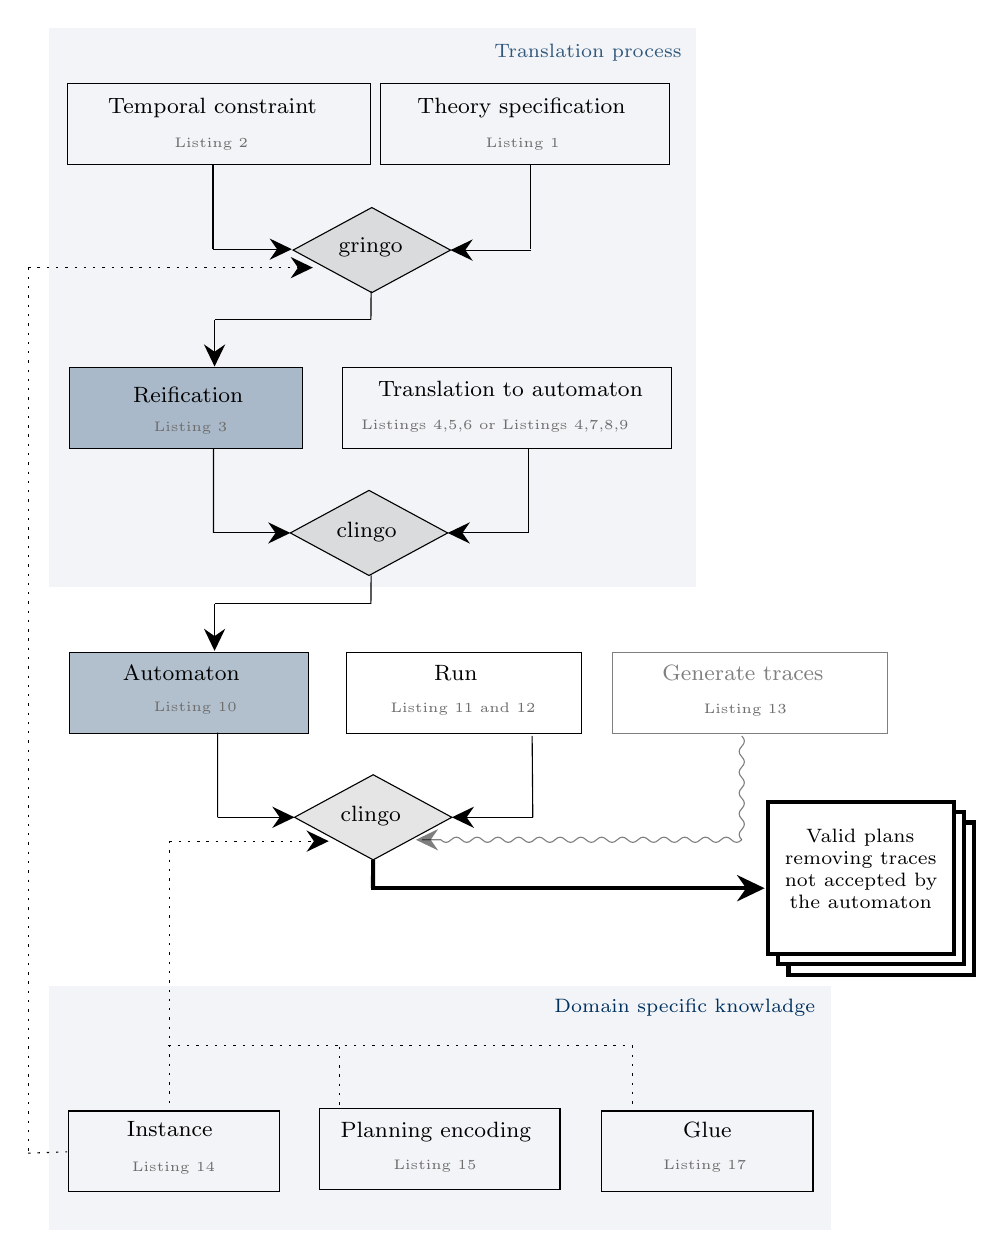
\begin{tikzpicture}[x=0.75pt,y=0.75pt,yscale=-1,xscale=1]
    %uncomment if require: \path (0,1205); %set diagram left start at 0, and has height of 1205
    
    %Shape: Rectangle [id:dp24788206372761257] 
    \draw  [fill={rgb, 255:red, 255; green, 255; blue, 255 }  ,fill opacity=1 ][line width=1.5]  (407,417) -- (496.55,417) -- (496.55,490.33) -- (407,490.33) -- cycle ;
    %Shape: Rectangle [id:dp28514107724578674] 
    \draw  [draw opacity=0][fill={rgb, 255:red, 0; green, 48; blue, 94 }  ,fill opacity=0.05 ][dash pattern={on 4.5pt off 4.5pt}] (50.5,495.67) -- (427.5,495.67) -- (427.5,613.33) -- (50.5,613.33) -- cycle ;
    %Shape: Rectangle [id:dp5077567162322292] 
    \draw  [draw opacity=0][fill={rgb, 255:red, 0; green, 48; blue, 94 }  ,fill opacity=0.05 ][dash pattern={on 4.5pt off 4.5pt}] (50.5,34.33) -- (362.5,34.33) -- (362.5,303.67) -- (50.5,303.67) -- cycle ;
    %Shape: Rectangle [id:dp8556117536304467] 
    \draw   (59.62,61) -- (205.42,61) -- (205.42,99.99) -- (59.62,99.99) -- cycle ;
    %Shape: Rectangle [id:dp3061835675075918] 
    \draw   (210.42,61) -- (349.62,61) -- (349.62,99.99) -- (210.42,99.99) -- cycle ;
    %Shape: Diamond [id:dp9415203890971041] 
    \draw  [fill={rgb, 255:red, 0; green, 0; blue, 0 }  ,fill opacity=0.1 ] (206.26,120.72) -- (244.17,141.22) -- (206.26,161.72) -- (168.34,141.22) -- cycle ;
    %Shape: Rectangle [id:dp0658574478056273] 
    \draw  [fill={rgb, 255:red, 0; green, 48; blue, 94 }  ,fill opacity=0.3 ] (60.62,198) -- (172.82,198) -- (172.82,236.99) -- (60.62,236.99) -- cycle ;
    %Shape: Rectangle [id:dp5420933852408244] 
    \draw   (192,198) -- (350.62,198) -- (350.62,236.99) -- (192,236.99) -- cycle ;
    %Shape: Diamond [id:dp7804185186549131] 
    \draw  [fill={rgb, 255:red, 0; green, 0; blue, 0 }  ,fill opacity=0.1 ] (204.91,257) -- (242.82,277.5) -- (204.91,298) -- (167,277.5) -- cycle ;
    %Shape: Rectangle [id:dp1579782039966966] 
    \draw  [fill={rgb, 255:red, 0; green, 48; blue, 94 }  ,fill opacity=0.3 ] (60.62,335) -- (175.82,335) -- (175.82,373.99) -- (60.62,373.99) -- cycle ;
    %Shape: Rectangle [id:dp21922696630916938] 
    \draw   (194,335) -- (307.15,335) -- (307.15,373.99) -- (194,373.99) -- cycle ;
    %Shape: Rectangle [id:dp26411591151258274] 
    \draw   (60,556) -- (161.82,556) -- (161.82,594.99) -- (60,594.99) -- cycle ;
    %Shape: Rectangle [id:dp9844105373777315] 
    \draw   (181,555) -- (296.93,555) -- (296.93,593.99) -- (181,593.99) -- cycle ;
    %Straight Lines [id:da9179998540863822] 
    \draw    (129.72,140.78) -- (164.72,140.78) ;
    \draw [shift={(167.72,140.78)}, rotate = 180] [fill={rgb, 255:red, 0; green, 0; blue, 0 }  ][line width=0.08]  [draw opacity=0] (10.72,-5.15) -- (0,0) -- (10.72,5.15) -- (7.12,0) -- cycle    ;
    %Straight Lines [id:da7912143421177068] 
    \draw    (283.17,141.22) -- (247.17,141.22) ;
    \draw [shift={(244.17,141.22)}, rotate = 360] [fill={rgb, 255:red, 0; green, 0; blue, 0 }  ][line width=0.08]  [draw opacity=0] (10.72,-5.15) -- (0,0) -- (10.72,5.15) -- (7.12,0) -- cycle    ;
    %Straight Lines [id:da8027967033545625] 
    \draw    (129.72,100.01) -- (129.72,140.78) ;
    %Straight Lines [id:da34160670813167726] 
    \draw    (282.72,100.01) -- (282.72,140.78) ;
    %Straight Lines [id:da568486742856372] 
    \draw    (205.83,174.67) -- (130.5,174.67) ;
    %Straight Lines [id:da9665051478374114] 
    \draw    (205.91,161) -- (205.83,174.67) ;
    %Straight Lines [id:da8317748002999547] 
    \draw    (281.82,277.5) -- (245.82,277.5) ;
    \draw [shift={(242.82,277.5)}, rotate = 360] [fill={rgb, 255:red, 0; green, 0; blue, 0 }  ][line width=0.08]  [draw opacity=0] (10.72,-5.15) -- (0,0) -- (10.72,5.15) -- (7.12,0) -- cycle    ;
    %Straight Lines [id:da4340309284116396] 
    \draw    (130,277.5) -- (164,277.5) ;
    \draw [shift={(167,277.5)}, rotate = 180] [fill={rgb, 255:red, 0; green, 0; blue, 0 }  ][line width=0.08]  [draw opacity=0] (10.72,-5.15) -- (0,0) -- (10.72,5.15) -- (7.12,0) -- cycle    ;
    %Straight Lines [id:da01308781139505788] 
    \draw    (129.99,236.73) -- (130,277.5) ;
    %Straight Lines [id:da018636812707615635] 
    \draw    (281.82,236.73) -- (281.82,277.5) ;
    %Straight Lines [id:da4867545297302681] 
    \draw  [dash pattern={on 0.84pt off 2.51pt}]  (108.72,426) -- (108.72,556.78) ;
    %Straight Lines [id:da3830532801993999] 
    \draw  [dash pattern={on 0.84pt off 2.51pt}]  (108.28,524.5) -- (332,524.5) ;
    %Straight Lines [id:da09223868766688892] 
    \draw  [dash pattern={on 0.84pt off 2.51pt}]  (190.5,525) -- (190.5,555.78) ;
    %Shape: Rectangle [id:dp5976304597228406] 
    \draw   (317,556) -- (418.82,556) -- (418.82,594.99) -- (317,594.99) -- cycle ;
    %Straight Lines [id:da4410590236065801] 
    \draw  [dash pattern={on 0.84pt off 2.51pt}]  (332,524.5) -- (332,556) ;
    %Straight Lines [id:da19225338333819464] 
    \draw  [dash pattern={on 0.84pt off 2.51pt}]  (40.72,149.67) -- (40.72,234) -- (40.72,576.33) ;
    %Straight Lines [id:da5024645482307678] 
    \draw  [dash pattern={on 0.84pt off 2.51pt}]  (40.72,149.67) -- (174.83,149.67) ;
    \draw [shift={(177.83,149.67)}, rotate = 180] [fill={rgb, 255:red, 0; green, 0; blue, 0 }  ][line width=0.08]  [draw opacity=0] (10.72,-5.15) -- (0,0) -- (10.72,5.15) -- (7.12,0) -- cycle    ;
    %Straight Lines [id:da5764659676991815] 
    \draw    (130.5,174.67) -- (130.5,194.33) ;
    \draw [shift={(130.5,197.33)}, rotate = 270] [fill={rgb, 255:red, 0; green, 0; blue, 0 }  ][line width=0.08]  [draw opacity=0] (10.72,-5.15) -- (0,0) -- (10.72,5.15) -- (7.12,0) -- cycle    ;
    %Straight Lines [id:da894604227602381] 
    \draw    (205.83,311.67) -- (130.5,311.67) ;
    %Straight Lines [id:da7188860332630708] 
    \draw    (130.5,311.67) -- (130.5,331.33) ;
    \draw [shift={(130.5,334.33)}, rotate = 270] [fill={rgb, 255:red, 0; green, 0; blue, 0 }  ][line width=0.08]  [draw opacity=0] (10.72,-5.15) -- (0,0) -- (10.72,5.15) -- (7.12,0) -- cycle    ;
    %Straight Lines [id:da3554509769994919] 
    \draw [line width=1.5]    (206.91,435) -- (206.83,448.67) ;
    %Straight Lines [id:da01324335735982407] 
    \draw  [dash pattern={on 0.84pt off 2.51pt}]  (40.72,576.33) -- (59.5,575.67) ;
    %Shape: Diamond [id:dp05782883080844736] 
    \draw  [fill={rgb, 255:red, 0; green, 0; blue, 0 }  ,fill opacity=0.1 ] (206.91,394) -- (244.82,414.5) -- (206.91,435) -- (169,414.5) -- cycle ;
    %Straight Lines [id:da09361882010550071] 
    \draw    (283.82,414.5) -- (247.82,414.5) ;
    \draw [shift={(244.82,414.5)}, rotate = 360] [fill={rgb, 255:red, 0; green, 0; blue, 0 }  ][line width=0.08]  [draw opacity=0] (10.72,-5.15) -- (0,0) -- (10.72,5.15) -- (7.12,0) -- cycle    ;
    %Straight Lines [id:da8326999325766362] 
    \draw    (132,414.5) -- (166,414.5) ;
    \draw [shift={(169,414.5)}, rotate = 180] [fill={rgb, 255:red, 0; green, 0; blue, 0 }  ][line width=0.08]  [draw opacity=0] (10.72,-5.15) -- (0,0) -- (10.72,5.15) -- (7.12,0) -- cycle    ;
    %Straight Lines [id:da35955432939448473] 
    \draw    (131.99,373.73) -- (132,414.5) ;
    %Straight Lines [id:da9796511600274105] 
    \draw    (283.5,375.33) -- (283.82,414.5) ;
    %Straight Lines [id:da08381943402202785] 
    \draw  [dash pattern={on 0.84pt off 2.51pt}]  (108.72,426) -- (182.5,426) ;
    \draw [shift={(185.5,426)}, rotate = 180] [fill={rgb, 255:red, 0; green, 0; blue, 0 }  ][line width=0.08]  [draw opacity=0] (10.72,-5.15) -- (0,0) -- (10.72,5.15) -- (7.12,0) -- cycle    ;
    %Straight Lines [id:da34272684140341236] 
    \draw [line width=1.5]    (391.5,448.67) -- (205.83,448.67) ;
    \draw [shift={(395.5,448.67)}, rotate = 180] [fill={rgb, 255:red, 0; green, 0; blue, 0 }  ][line width=0.08]  [draw opacity=0] (13.4,-6.43) -- (0,0) -- (13.4,6.44) -- (8.9,0) -- cycle    ;
    %Straight Lines [id:da38816660652930635] 
    \draw    (205.91,298) -- (205.83,311.67) ;
    %Shape: Rectangle [id:dp31370535660350696] 
    \draw  [color={rgb, 255:red, 0; green, 0; blue, 0 }  ,draw opacity=0.5 ] (322.15,335) -- (454.62,335) -- (454.62,373.99) -- (322.15,373.99) -- cycle ;
    %Straight Lines [id:da9731404355029183] 
    \draw [color={rgb, 255:red, 0; green, 0; blue, 0 }  ,draw opacity=0.5 ]   (384.5,375.33) .. controls (386.17,377) and (386.17,378.66) .. (384.5,380.33) .. controls (382.83,382) and (382.83,383.66) .. (384.5,385.33) .. controls (386.17,387) and (386.17,388.66) .. (384.5,390.33) .. controls (382.83,392) and (382.83,393.66) .. (384.5,395.33) .. controls (386.17,397) and (386.17,398.66) .. (384.5,400.33) .. controls (382.83,402) and (382.83,403.66) .. (384.5,405.33) .. controls (386.17,407) and (386.17,408.66) .. (384.5,410.33) .. controls (382.83,412) and (382.83,413.66) .. (384.5,415.33) .. controls (386.17,417) and (386.17,418.66) .. (384.5,420.33) .. controls (382.83,422) and (382.83,423.66) .. (384.5,425.33) -- (384.5,425.33) -- (384.5,425.33) ;
    %Straight Lines [id:da6224255621877544] 
    \draw [color={rgb, 255:red, 0; green, 0; blue, 0 }  ,draw opacity=0.5 ]   (384.5,425.33) .. controls (382.83,427) and (381.17,427) .. (379.5,425.33) .. controls (377.83,423.66) and (376.17,423.66) .. (374.5,425.33) .. controls (372.83,427) and (371.17,427) .. (369.5,425.33) .. controls (367.83,423.66) and (366.17,423.66) .. (364.5,425.33) .. controls (362.83,427) and (361.17,427) .. (359.5,425.33) .. controls (357.83,423.66) and (356.17,423.66) .. (354.5,425.33) .. controls (352.83,427) and (351.17,427) .. (349.5,425.33) .. controls (347.83,423.66) and (346.17,423.66) .. (344.5,425.33) .. controls (342.83,427) and (341.17,427) .. (339.5,425.33) .. controls (337.83,423.66) and (336.17,423.66) .. (334.5,425.33) .. controls (332.83,427) and (331.17,427) .. (329.5,425.33) .. controls (327.83,423.66) and (326.17,423.66) .. (324.5,425.33) .. controls (322.83,427) and (321.17,427) .. (319.5,425.33) .. controls (317.83,423.66) and (316.17,423.66) .. (314.5,425.33) .. controls (312.83,427) and (311.17,427) .. (309.5,425.33) .. controls (307.83,423.66) and (306.17,423.66) .. (304.5,425.33) .. controls (302.83,427) and (301.17,427) .. (299.5,425.33) .. controls (297.83,423.66) and (296.17,423.66) .. (294.5,425.33) .. controls (292.83,427) and (291.17,427) .. (289.5,425.33) .. controls (287.83,423.66) and (286.17,423.66) .. (284.5,425.33) .. controls (282.83,427) and (281.17,427) .. (279.5,425.33) .. controls (277.83,423.66) and (276.17,423.66) .. (274.5,425.33) .. controls (272.83,427) and (271.17,427) .. (269.5,425.33) .. controls (267.83,423.66) and (266.17,423.66) .. (264.5,425.33) .. controls (262.83,427) and (261.17,427) .. (259.5,425.33) .. controls (257.83,423.66) and (256.17,423.66) .. (254.5,425.33) .. controls (252.83,427) and (251.17,427) .. (249.5,425.33) .. controls (247.83,423.66) and (246.17,423.66) .. (244.5,425.33) .. controls (242.83,427) and (241.17,427) .. (239.5,425.33) -- (238.5,425.33) -- (230.5,425.33) ;
    \draw [shift={(227.5,425.33)}, rotate = 360] [fill={rgb, 255:red, 0; green, 0; blue, 0 }  ,fill opacity=0.5 ][line width=0.08]  [draw opacity=0] (10.72,-5.15) -- (0,0) -- (10.72,5.15) -- (7.12,0) -- cycle    ;
    %Shape: Rectangle [id:dp4398006989421265] 
    \draw  [fill={rgb, 255:red, 255; green, 255; blue, 255 }  ,fill opacity=1 ][line width=1.5]  (402,412) -- (491.55,412) -- (491.55,485.33) -- (402,485.33) -- cycle ;
    %Shape: Rectangle [id:dp7390603575053865] 
    \draw  [fill={rgb, 255:red, 255; green, 255; blue, 255 }  ,fill opacity=1 ][line width=1.5]  (397,407) -- (486.55,407) -- (486.55,480.33) -- (397,480.33) -- cycle ;
    
    % Text Node
    \draw (78,66.93) node [anchor=north west][inner sep=0.75pt]  [font=\footnotesize] [align=left] {Temporal constraint};
    % Text Node
    \draw (227,66.93) node [anchor=north west][inner sep=0.75pt]  [font=\footnotesize] [align=left] {Theory specification};
    % Text Node
    \draw (189,133.93) node [anchor=north west][inner sep=0.75pt]  [font=\footnotesize] [align=left] {gringo};
    % Text Node
    \draw (90,205.93) node [anchor=north west][inner sep=0.75pt]  [font=\footnotesize] [align=left] {Reification};
    % Text Node
    \draw (208,202.93) node [anchor=north west][inner sep=0.75pt]  [font=\footnotesize] [align=left] {Translation to automaton};
    % Text Node
    \draw (188,270.93) node [anchor=north west][inner sep=0.75pt]  [font=\footnotesize] [align=left] {clingo};
    % Text Node
    \draw (85,339.93) node [anchor=north west][inner sep=0.75pt]  [font=\footnotesize] [align=left] {Automaton};
    % Text Node
    \draw (235,339.93) node [anchor=north west][inner sep=0.75pt]  [font=\footnotesize] [align=left] {Run};
    % Text Node
    \draw (87,559.93) node [anchor=north west][inner sep=0.75pt]  [font=\footnotesize] [align=left] {Instance};
    % Text Node
    \draw (190,559.93) node [anchor=north west][inner sep=0.75pt]  [font=\footnotesize] [align=left] {Planning encoding};
    % Text Node
    \draw (404,418.93) node [anchor=north west][inner sep=0.75pt]  [font=\scriptsize] [align=left] {\begin{minipage}[lt]{54.78804595947266pt}\setlength\topsep{0pt}
    \begin{center}
    Valid plans\\removing traces\\not accepted by \\the automaton
    \end{center}
    
    \end{minipage}};
    % Text Node
    \draw (355,559.93) node [anchor=north west][inner sep=0.75pt]  [font=\footnotesize] [align=left] {Glue};
    % Text Node
    \draw (190,407.93) node [anchor=north west][inner sep=0.75pt]  [font=\footnotesize] [align=left] {clingo};
    % Text Node
    \draw (293,500.6) node [anchor=north west][inner sep=0.75pt]  [font=\scriptsize,color={rgb, 255:red, 0; green, 48; blue, 94 }  ,opacity=1 ] [align=left] {Domain specific knowladge};
    % Text Node
    \draw (264,40.6) node [anchor=north west][inner sep=0.75pt]  [font=\scriptsize,color={rgb, 255:red, 0; green, 48; blue, 94 }  ,opacity=0.8 ] [align=left] {Translation process};
    % Text Node
    \draw (345,339.93) node [anchor=north west][inner sep=0.75pt]  [font=\footnotesize,color={rgb, 255:red, 0; green, 0; blue, 0 }  ,opacity=0.5 ] [align=left] {Generate traces};
    % Text Node
    \draw (110,85.93) node [anchor=north west][inner sep=0.75pt]  [font=\tiny,color={rgb, 255:red, 110; green, 108; blue, 108 }  ,opacity=1 ] [align=left] {Listing 2};
    % Text Node
    \draw (260,85.93) node [anchor=north west][inner sep=0.75pt]  [font=\tiny,color={rgb, 255:red, 110; green, 108; blue, 108 }  ,opacity=1 ] [align=left] {Listing 1};
    % Text Node
    \draw (100,222.93) node [anchor=north west][inner sep=0.75pt]  [font=\tiny,color={rgb, 255:red, 110; green, 108; blue, 108 }  ,opacity=1 ] [align=left] {Listing 3};
    % Text Node
    \draw (100,357.93) node [anchor=north west][inner sep=0.75pt]  [font=\tiny,color={rgb, 255:red, 110; green, 108; blue, 108 }  ,opacity=1 ] [align=left] {Listing 10};
    % Text Node
    \draw (200,221.93) node [anchor=north west][inner sep=0.75pt]  [font=\tiny,color={rgb, 255:red, 110; green, 108; blue, 108 }  ,opacity=1 ] [align=left] {Listings 4,5,6 or Listings 4,7,8,9};
    % Text Node
    \draw (214,357.93) node [anchor=north west][inner sep=0.75pt]  [font=\tiny,color={rgb, 255:red, 110; green, 108; blue, 108 }  ,opacity=1 ] [align=left] {Listing 11 and 12};
    % Text Node
    \draw (365,358.93) node [anchor=north west][inner sep=0.75pt]  [font=\tiny,color={rgb, 255:red, 110; green, 108; blue, 108 }  ,opacity=1 ] [align=left] {Listing 13};
    % Text Node
    \draw (89.5,579.6) node [anchor=north west][inner sep=0.75pt]  [font=\tiny,color={rgb, 255:red, 110; green, 108; blue, 108 }  ,opacity=1 ] [align=left] {Listing 14};
    % Text Node
    \draw (215.5,578.6) node [anchor=north west][inner sep=0.75pt]  [font=\tiny,color={rgb, 255:red, 110; green, 108; blue, 108 }  ,opacity=1 ] [align=left] {Listing 15};
    % Text Node
    \draw (345.5,578.6) node [anchor=north west][inner sep=0.75pt]  [font=\tiny,color={rgb, 255:red, 110; green, 108; blue, 108 }  ,opacity=1 ] [align=left] {Listing 17};
    
    
    \end{tikzpicture}
    
    

    


    \caption{The diagram shows an overview of the workflow for the integration. All components consist of ASP encodings. Components marked in dark blue are generated by the system. Dotted lines correspond to the inclusion of elements from the specific application domain. Lastly, the component in grey refers to the optional task of trace generation. }
    \label{workflow}
\end{figure}



\subsection{Theory enhanced ASP solving  }


The system $\clingo$ can be extended with theory-specific reasoning enabling a complementary behavior for the desired functionality \cite{kascwa17a}. In this thesis, we do not explain the semantic principles of theory solving, but instead we focus only on how $\clingo$'s input language can be customized with theory-specific constructs as part of its underlying grounder $\gringo$. This feature allows us to include the syntax required for temporal and dynamic formulas in the modeling language. We summarize the designated characters for every operator in tables 1 and 2. Furthermore, this extension is merged into the grounding process, thus proving the means for the use of variables and generalized concepts in our formulas.

\vspace{10px}
\begin{minipage}{.40\textwidth}
    \centering
        \begin{tabular}{|l|l|l|}
            \hline
            \textbf{Operator} & \textbf{Symbol} & \textbf{\clingo} \\
            \hline
            Not & $\neg$ & \texttt{\textasciitilde} \\
            Next & $\Next$ & \texttt{>} \\
            Week Next & $\wnext$ & \texttt{>:} \\
            And & $\wedge$ & \texttt{\&} \\
            Or & $\vee$ & \texttt{$\|$} \\
            Until & $\until$ & \texttt{>?} \\
            Release & $\release$ & \texttt{>*} \\
            \hline
        \end{tabular}
        \captionof{table}{Symbols incorporated to $\clingo$ for $\LTLf$.}
\end{minipage}
\hspace{25px}
\begin{minipage}{.40\textwidth}
    \centering

        \begin{tabular}{|l|l|l|}
            \hline
            \textbf{Operator} & \textbf{Symbol} & \textbf{\clingo} \\
            \hline
            Not & $\neg$ & \texttt{\textasciitilde} \\
            Test & $?$ & \texttt{?} \\
            Star & $\ast$ & \texttt{*} \\
            Choice & $+$ & \texttt{+} \\
            Sequence & $;$ & \texttt{;;} \\
            Diamond & $\langle \rangle$ & \texttt{.>?} \\
            Box & $\dalways{ }$ & \texttt{.>*} \\
            \hline
        \end{tabular}
        \captionof{table}{Symbols incorporated to $\clingo$ for $\LDLf$.}
\end{minipage}
\vspace{10px}
    

The theory specifications characterizing the grammars for temporal and dynamic formulas are encoded by defining a theory language. We illustrate this with the encoding for $\LTLf$ in Listing 1, similar to that of  $\LDLf$. 


\begin{center}
    \begin{lstlisting}[] 
#theory tel {
    tel_formula  {
        &   : 7, unary;         % prefix for boolean constants
        ~   : 5, unary;         % negation
        >   : 5, unary;         % next
        >:  : 5, unary;         % weak next
        &   : 3, binary, left;  % and
        |   : 2, binary, left;  % or
        >?  : 4, binary, left;  % until
        >*  : 4, binary, left   % release
    };
    &tel/0 : tel_formula, body
}.
    \end{lstlisting}
    \captionof{lstlisting}{Theory specification for temporal formulas}
\end{center}

The theory language for characterizing a temporal formula is defined in lines 2-12, preceded by the directive \texttt{\#theory}. 
Lines 2-11 represent a \emph{theory term definition} of the form $t \;\{D_1;...;D_n\}$, where each $D_i$ is a \emph{theory operator definition} corresponding to the operators in the grammar. Theory operators can be unary or binary, where the second type is further characterized by a right or left associativity. Finally, line 12 describes a \emph{theory atom} constructed with the theory term definition \texttt{tel\_formula}. The theory atom is only allowed to appear in the body of a rule by using the occurrence type \texttt{body}.\footnote{We only require formulas in the body since we are restricted to integrity constraints.}

\begin{example}
    The formula $\Next a \wedge (b \until a)$ from Example 6 can be encoded in an integrity constraint using the theory specification defined above. 
    \begin{center}
        \begin{lstlisting}[] 
:- not &tel{ > a & (b >? a) }.
        \end{lstlisting}
        \captionof{lstlisting}{Example of temporal constraint}
    \end{center}

\end{example}

Once the grounding process is completed, $\clingo$ represents the ground program in an intermediate language using the \emph{aspif} format \cite{kascwa17a}, where a ground logic program is mapped into a sequence of lines of aspif statements describing all rules and constructs by means of numbers. A fraction of this representation is addressed to the theory-specific part, outputting a linear representation of the abstract syntax tree for the given theory expression. Since its representation based on numbers doesn't make the output humanly readable, one of the options provided by $\gringo$ is a reified output where aspif statements are expressed in the form of facts. Using this feature, we can then represent the abstract syntax tree of the formulas described in our theory specification as a set of facts. 

\begin{example}
    Below we show the facts from the reified output corresponding to the theory expression of the previous example, namely \texttt{\&tel\{ > a \& (b >? a) \}}
    \begin{center}
        \begin{lstlisting}[] 
theory_string(0,"tel").
theory_string(3,"a").
theory_string(2,">").
theory_tuple(0).
theory_tuple(0,0,3).
theory_function(4,2,0).
theory_string(6,"b").
theory_string(5,">?").
theory_tuple(1).
theory_tuple(1,0,6).
theory_tuple(1,1,3).
theory_function(7,5,1).
theory_string(1,"&").
theory_tuple(2).
theory_tuple(2,0,4).
theory_tuple(2,1,7).
theory_function(8,1,2).
theory_tuple(3).
theory_tuple(3,0,8).
literal_tuple(1).
theory_element(0,3,1).
theory_element_tuple(0).
theory_element_tuple(0,0).
theory_atom(1,0,0).
        \end{lstlisting}
        \captionof{lstlisting}{Section of reified output of grounding Listing 1 and 2 via ‘\texttt{gringo --output=reify listing-1.lp listing-2.lp}’}
    \end{center}
\end{example}

All the theory-specific facts we obtain with this process have as first argument an identifier, where the identifiers can't be repeated between predicates  \textit{theory\_function}, \textit{theory\_string} and \textit{theory\_number}. The rest of the arguments depend on the construct, most arguments refer to the relationship with its children in the abstract syntax tree (AST) via identifiers, while others correspond to a value in the form of string or number for \textit{theory\_string} and \textit{theory\_number} respectively. In the case of predicate \textit{theory\_tuple}, which defines tuples that are then passed to a function (with or without name), the second argument refers to the index of the tuple containing the element described by the identifier in the third argument. The association between formulas and identifiers has a one-to-one correspondence, hence a subformula $\psi$ is associated with a unique identifier which is reused in every appearance of $\psi$. 


\begin{example}
    Here we show the abstract syntax tree described in Listing 3 for formula $\varphi= \Next a \wedge (b \until a)$. The tree on the left side considers the ids of the \textit{theory\_string} predicates, whereas the one in the right uses the ids from \textit{theory\_function} in the nodes marked in blue. We can notice how id number $3$ is used to identify $a$ in both subtrees.
    \begin{multicols*}{2}
        
    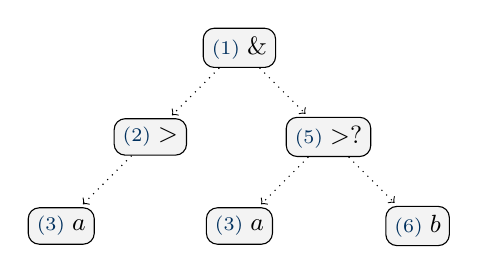
\begin{tikzpicture}[shorten >=1.5pt,node distance=1.6cm,on grid,auto]
    \small
    \tikzstyle{tree_node}=[rounded corners,fill={rgb:black,1;white,20},font=\small,draw=black]
    \node[tree_node]  (and)                 {\textcolor{darkblue}{\scriptsize{(1)}}$\;\&$};
    \node[tree_node]  (next) [below left of =and]                {\textcolor{darkblue}{\scriptsize{(2)}}$\;>$};
    \node[tree_node]  (until)[below right of =and]               {\textcolor{darkblue}{\scriptsize{(5)}}$\;>?$};
    
    \node[tree_node]  (a)[below left of =next]               {\textcolor{darkblue}{\scriptsize{(3)}}$\;a$};
    

\node[tree_node]  (b)[below right of =until]               {\textcolor{darkblue}{\scriptsize{(6)}}$\;b$};
\node[tree_node]  (a_2)[below left of =until]               {\textcolor{darkblue}{\scriptsize{(3)}}$\;a$};

\path[->,dotted]
(and) edge                node {}  (next) 
(and) edge               node {}  (until) 
(next) edge                node {}  (a)
(until) edge                node {}  (b)
(until) edge                node {}  (a_2);

\end{tikzpicture}
    \captionof{figure}{AST using ids for strings}

    
    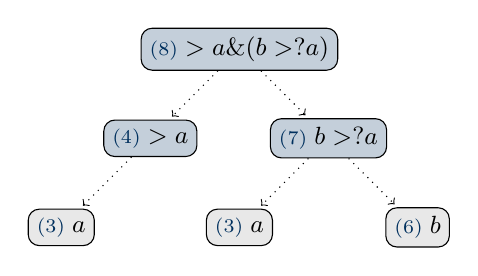
\begin{tikzpicture}[shorten >=1.5pt,node distance=1.6cm,on grid,auto]
        \small
        \tikzstyle{tree_node}=[rounded corners,fill={rgb:black,1;white,10},font=\small,draw=black]
        \tikzstyle{tree_node_fun}=[rounded corners,fill={rgb:darkblue,3;white,10},font=\small,draw=black]
        \node[tree_node_fun]  (and)                 {\textcolor{darkblue}{\scriptsize{(8)}}$\;> a \& (b >? a)$};
        \node[tree_node_fun]  (next) [below left of =and]                {\textcolor{darkblue}{\scriptsize{(4)}}$\;> a$};
    \node[tree_node_fun]  (until)[below right of =and]               {\textcolor{darkblue}{\scriptsize{(7)}}$\;b >? a$};
    
    \node[tree_node]  (a)[below left of =next]               {\textcolor{darkblue}{\scriptsize{(3)}}$\;a$};
    
    \node[tree_node]  (b)[below right of =until]               {\textcolor{darkblue}{\scriptsize{(6)}}$\;b$};
    \node[tree_node]  (a_2)[below left of =until]               {\textcolor{darkblue}{\scriptsize{(3)}}$\;a$};
    
    \path[->,dotted]
    (and) edge                node {}  (next) 
     (and) edge               node {}  (until) 
    (next) edge                node {}  (a)
    (until) edge                node {}  (b)
    (until) edge                node {}  (a_2);
    
    \end{tikzpicture}
    \captionof{figure}{AST using ids for functions}


\end{multicols*}
\end{example}


\subsection{Automaton translation  }

Given the set of facts from the reification of a temporal formula, we now proceed to generate the equivalent automaton. First, we must single out all propositions used in the formula which will correspond to the alphabet $\A$. Propositions can be characterized by their corresponding identifier on the theory facts as it is done in the encoding below. 

\begin{center}
    \begin{lstlisting}[] 
pos_prop_id(ID) :- theory_function(ID,ID_O,ID_T),
                   theory_string(ID_O,P), 
                   not operator(P),
                   not reserved_words(P).

pos_prop_id(ID) :- theory_string(ID,P),
                   not operator(P), 
                   not reserved_words(P).

prop_id(ID) :- pos_prop_id(ID), 
               #count{1,ID_P: theory_function(ID_P, _, ID_T),
                              theory_tuple(ID_T,0..MAX,ID),
                              not pos_prop_id(ID_P)} > 0, 
               #max{D:theory_tuple(_,D,_)} = MAX.

used_id(ID) :- theory_string(ID,S), S != "last".
used_id(ID) :- theory_function(ID,IDS,_), 
               theory_string(IDS,S), S != "last".
last_id(MID+1) :- #max{ID:used_id(ID)} = MID.
theory_string(ID,"last") :- last_id(ID).

    \end{lstlisting}
    \captionof{lstlisting}{Encoding handling propositions}
\end{center}

The identifier used for a proposition is selected depending on whether the proposition comes from a nested predicate, such as $a(b)$, or one with arity 0 like $a$.
We use the identifier from $theory\_function$ in the case of predicates with arity grater than 0 (lines 1-4), corresponding to either functions or nested predicates (marked in blue on Figure 3).
On the other hand, for those with arity 0, we use the identifier from $theory\_string$ (lines 6-8). 
We exclude theory facts describing operators of our grammar and reserved words, saved in predicates \texttt{operator/1}\footnote{We use \texttt{p/i} to describe a predicate with name $p$ and arity $i$} and \texttt{reserved\_words/1}, respectively. 
Additionally, we remove terms which only appear as part of the arguments of other propositions (lines 10-14). 
This will allow us, for instance, to consider only $b(a)$ in our alphabet without considering $a$.
To achieve this, the rule uses two types of aggregates \cite{potasscoManual}, which are modeling constructs that let us from groups of selected items subject to conditions. 
In this case, aggregate \texttt{\#count} from line 11, will count the number of times a possible proposition, with id \texttt{ID}, appears in the arguments of another possible proposition with id \texttt{ID\_P}, and make sure this number is 0. 
In line 14 we use the aggregate \texttt{\#max} to find the largest arity, in order to limit the previous search.


Moreover, we manually include the special proposition $\mathit{last}$ required in our translation (lines 16-20). Predicate \texttt{used\_id/1} gathers all used identifiers in lines 16 and 17. Line 19 computes the next free identifier, while line 20 incorporates it as if it were part of the reified output.

% TODO id_map define, when it is final

The next step consists of defining the set of states and the transition function of the automaton. 
Different approaches were taken for each logic due to implementation restrictions. Let us now go into the details for each specific logic. 



\subsubsection{States and transitions for $\LTLf$}

As seen before, the translation from a temporal formula $\varphi$ into an alternating automaton defines the set of states using a special closure $cl(\varphi)$. 
In this definition, a special treatment is given to formulas $\varphi_1\release\varphi_2$ and $\varphi_1\until\varphi_2$. 
However, we can limit the closure to only the subformulas of $\varphi$, consequently reducing the set of states. 
This is achieved by unfolding the transitions of these two operators with the case analysis corresponding to the next and weak next operators respectively. 

Working only with the subformulas gives us the advantage of using the identifiers from the reified output as states. Such decision is based on the key observation that all subformulas are given a unique identifier appearing in the $theory\_function$ predicate, as it is illustrated in the AST in Figure 3. 


\begin{center}
    \begin{lstlisting}[] 
state(ID) :- theory_function(ID,ID_O,ID_T),
             theory_string(ID_O,P), 
             operator(P).

state(ID):- prop_id(ID).

initial_state(ID) :- theory_atom(ID_A,ID_O,ID_E),
                     theory_string(ID_O,"tel"),
                     theory_element(ID_E,ID_T,_),
                     theory_tuple(ID_T,0,ID).
    \end{lstlisting}
    \captionof{lstlisting}{Encoding defining states from temporal formulas}
\end{center}

Lines 1-3 collect all functions, representing subformulas, from the reified output using the operators of the grammar. Line 5 includes propositions, computed in Listing 4, as part of the states. Finally, line 7 defines the initial state of the automaton using special theory-specific facts. 

Regarding the transition function, both logics encode it base of the transition system with a predicate \texttt{delta/2}, composed by a state and an extended positive Boolean formula. Considered in these extended positive Boolean formulas is also the case analysis over the current interpretation. 
Such formulas are constructed with predicates: \texttt{pbf\_true/0} and \texttt{pbf\_false/0} for Boolean constants; \texttt{pbf\_and/2} and \texttt{pbf\_or/2} connecting two formulas; \texttt{pbf\_state/1} where the the argument is a state; and lastly \texttt{pbf\_if/3} used to represent the case analysis based on the propositional identifier as first argument. Listing 6 is a representative part of the encoding constructing the transition function for temporal formulas. The definitions for the remaining operators are analogous to the ones presented. 

\begin{center}
    \begin{lstlisting}[] 
% Proposition
delta(ID ,pbf_if(ID,pbf_true,pbf_false)) :- 
        prop_id(ID).

% True (False)
delta(ID ,pbf_true) :-
        theory_function(ID,ID_O,ID_T),
        theory_string(ID_O,"&"),
        theory_tuple(ID_T,0,ID_L),
        theory_string(ID_L,"true").

% Negation
delta(ID ,pbf_if(ID_L,pbf_false,pbf_true)) :- 
        theory_function(ID,ID_O,ID_T),
        theory_string(ID_O,"~"),
        theory_tuple(ID_T,0,ID_L).
        
% Next (Weak next)
delta(ID ,pbf_if(ID_LAST,pbf_false,pbf_state(ID_L))) :-
        theory_function(ID,ID_O,ID_T),
        theory_string(ID_O,">"),
        theory_tuple(ID_T,0,ID_L),
        last_id(ID_LAST).

% And (Or)
delta(ID ,pbf_and(PBF_L,PBF_R)) :-
        theory_function(ID,ID_O,ID_T),
        theory_string(ID_O,"&"),
        theory_tuple(ID_T,0,ID_L),
        theory_tuple(ID_T,1,ID_R),
        delta(ID_L,PBF_L),
        delta(ID_R,PBF_R).

% Until (Release)
delta(ID ,pbf_or(PBF_R,pbf_and(PBF_L,pbf_if(ID_LAST,pbf_false,pbf_state(ID))))):-
        theory_function(ID,ID_O,ID_T),
        theory_string(ID_O,">?"),
        theory_tuple(ID_T,0,ID_L),
        theory_tuple(ID_T,1,ID_R),
        delta(ID_L,PBF_L),
        delta(ID_R,PBF_R),
        last_id(ID_LAST).
\end{lstlisting}
\captionof{lstlisting}{Representative part of the encoding defining the transition function for temporal formulas}
\end{center}

\subsubsection{States and transitions for $\LDLf$}


Unlike for $\LTLf$, in the case of dynamic formulas we are forced to compute the closure of the formula in order to construct the set of states. During the construction of the states, we can't longer identify them with a number, as it is impossible to generate new identifiers for each formula in the closure using only ASP. Therefore, states will be identified in $\LDLf$ by a predicate. To achieve this we first map the ids from the reified linear format into a representation based on nested predicates, as shown in Listing 7\footnote{We include the negation to simplify syntax.}. 

\begin{center}
    \begin{lstlisting}[] 
% Proposition
map_id_to_predicate(ID,prop(ID)) :- 
        prop_id(ID).

% Top (Bottom)
map_id_to_predicate(ID,top) :-                                                        
        theory_function(ID,ID_O,ID_T), 
        theory_string(ID_O,"&"),
        theory_tuple(ID_T,0,ID_L),
        theory_string(ID_L,"true").

% Negation
map_id_to_predicate(ID,neg(FL)) :-                                                        
        theory_function(ID,ID_O,ID_T), 
        theory_string(ID_O,"~"),
        theory_tuple(ID_T,0,ID_L),
        map_id_to_predicate(ID_L,FL).

% Diamond (Box) (Box (Box))
map_id_to_predicate(ID,diamond(FL,FR)) :-
        theory_function(ID,ID_O,ID_T),
        theory_string(ID_O,".>?"),
        theory_tuple(ID_T,0,ID_L),
        theory_tuple(ID_T,1,ID_R),
        map_id_to_predicate(ID_L,FL), 
        map_id_to_predicate(ID_R,FR).

% Test Path (Star Path)
map_id_to_predicate(ID,test(FL)) :-                                                   
        theory_function(ID,ID_O,ID_T), 
        theory_string(ID_O,"?"),
        theory_tuple(ID_T,0,ID_L),
        map_id_to_predicate(ID_L,FL).

% Sequence Path (Choice Path)
map_id_to_predicate(ID,sequence(FL,FR)) :-                                                   
        theory_function(ID,ID_O,ID_T), 
        theory_string(ID_O,";;"),
        theory_tuple(ID_T,0,ID_L),
        theory_tuple(ID_T,1,ID_R),
        map_id_to_predicate(ID_L,FL), 
        map_id_to_predicate(ID_R,FR).
\end{lstlisting}
\captionof{lstlisting}{Encoding defining the mapping between ids and nested predicates for dynamic formulas}
\end{center}


Using the new representation, we construct the set of states based on the closure.
For this process, we use predicate \texttt{dynamic\_formula/1}, containing only the nested predicates for dynamic formulas saved in \texttt{map\_id\_to\_predicate/2}, while excluding the path expressions. The encoding is provided in Listing 8, where Line 1 includes all dynamic formulas in the closure, Line 3 includes the negation of propositions, lines 5 to 17 define the closure for the diamond operator (analogous the box operator), and finally line 19 defines the set of states derived from the closure. 

\begin{center}
    \begin{lstlisting}[] 
closure(F) :- dynamic_formula(F).

closure(neg(prop(ID))) :- closure(prop(ID)).

closure(diamond(X,Z)) :- 
        closure(diamond(choice(X,Y),Z)).

closure(diamond(Y,Z)) :- 
        closure(diamond(choice(X,Y),Z)).

closure(diamond(X,diamond(Y,Z))) :- 
        closure(diamond(sequence(X,Y),Z)).

closure(diamond(X,diamond(star(X),Z))) :- 
        closure(diamond(star(X),Z)).

closure(Z) :- closure(diamond(_,Z)).

state(F) :- closure(F).
\end{lstlisting}
\captionof{lstlisting}{Encoding defining closure and states for dynamic formulas}
\end{center}



% Thus, we must identify them in a different way, in this case by transforming the reified linear format into a representation based on nested predicates. 


It is also relevant to recall that negation was defined as syntactic sugar in our grammar and therefore can be fully eliminated. 
However, for simplicity, we include it in the implementation only before atoms. With the new representation of states, the definition of the transition function is straight-forward. Nonetheless, we show part of this encoding in Listing 9.


\begin{center}
    \begin{lstlisting}[] 
% Proposition
delta(prop(A),pbf_if(A,pbf_true,pbf_false)) :- 
        state(prop(A)).

% Negation
delta(neg(prop(A)),pbf_if(A,pbf_false,pbf_true)) :- 
        state(neg(prop(A))).

% Diamond Test (Box Test)
delta(diamond(test(F1),F2),pbf_and(BF1,BF2)) :- 
        state(diamond(test(F1),F2)), 
        delta(F1,BF1), 
        delta(F2,BF2).

% Diamond Step (Box Step)
delta(diamond(top,F),pbf_if(LAST,pbf_false,pbf_state(F))) :- 
        state(diamond(top,F)),
        last_id(LAST).

% Diamond Choice  (Box Choice)
delta(diamond(choice(P1,P2),F),pbf_or(BF1,BF2)) :- 
        state(diamond(choice(P1,P2),F)),
        delta(diamond(P1,F),BF1), 
        delta(diamond(P2,F),BF2).

% Diamond Sequence (Box Sequence)
delta(diamond(sequence(P1,P2),F),B) :- 
        state(diamond(sequence(P1,P2),F)),
        delta(diamond(P1,diamond(P2,F)),B).

% Diamond Star (Box Star)
delta(diamond(star(test(P)),F),B) :- 
        state(diamond(star(test(P)),F)), 
        delta(F,B).

is_test(test(P)):-state(diamond(star(test(P)),F)).
delta(diamond(star(P),F),pbf_or(BF,B)) :- 
        state(diamond(star(P),F)),
        delta(diamond(P,diamond(star(P),F)),B),
        delta(F,BF),
        not is_test(P).
\end{lstlisting}
\captionof{lstlisting}{Encoding defining transition function for $\LDLf$}
\end{center}


After calling $\clingo$ with the given encodings for each logic, we complete the translation process. The resulting declarative representation of the automaton, is a list of facts composed by predicates \texttt{state/1}, \texttt{initial\_state/1} and \texttt{delta/2}. Additional predicates \texttt{id\_prop/1} and \texttt{id\_last/1} are also saved, since they are needed to run traces by the automaton. The representation is unified between both logics, differing only in the way states are identified, thus making the rest of the implementation independent of the type of logic. 

\begin{example}[Automaton declarative representation]
        
        \begin{center}
                \begin{lstlisting}[] 
initial_state(8).
prop_id(3).
prop_id(6).
state(3).
state(6).
state(4).
state(7).
state(8).
last_id(9).
delta(3,pbf_if(3,pbf_true,pbf_false)).
delta(6,pbf_if(6,pbf_true,pbf_false)).
delta(4,pbf_if(9,pbf_false,pbf_state(3))).
delta(7,pbf_or(pbf_if(3,pbf_true,pbf_false),
        pbf_and(pbf_if(6,pbf_true,pbf_false),
        pbf_if(9,pbf_false,pbf_state(7))))).
delta(8,pbf_and(pbf_if(9,pbf_false,pbf_state(3)),
        pbf_or(pbf_if(3,pbf_true,pbf_false),
        pbf_and(pbf_if(6,pbf_true,pbf_false),
        pbf_if(9,pbf_false,pbf_state(7)))))).

                \end{lstlisting}
        \captionof{lstlisting}{Example of the automaton representation for the running example from Listing 2. The identifies of the states correspond to those from Listing 3.}
        \end{center}
\end{example}


\subsection{Accepted runs of an automaton  }

We now go ahead with the verification of traces using the automaton. Traces can be either randomly generated, explicitly defined as facts or computed as part of a planning problem, the last case is addressed in a following section. We describe traces using a predicate \texttt{in\_trace\_at(ID,T)} \footnote{We avoid the use of usual propositions \textit{holds} and \textit{occurs}, because from the point of view of the automaton there is no difference between actions and fluents. Furthermore, such predicates are likely to have already been used in the planning domain, causing inconsistencies.} stating that the proposition with id \textit{ID} is in the trace at time point $T$.

Further consideration was needed for the special proposition $\mathit{last}$. Like for most dynamic scenarios, we require a fixed horizon as part of the parameters for solving. Such horizon defines the length of all traces, therefore, determining the time step where the special proposition $\mathit{last}$ holds, encoded in the rule \texttt{in\_trace\_at(ID,horizon) :- last\_id(ID).}.

For the evaluation of traces, we construct runs as $S-$labeled trees. We introduce predicate \texttt{node\_run/3}, where the first argument is either a Boolean constant, represented by \texttt{true} and \texttt{false}, or \texttt{state\_id(ID)} mapping the node to its corresponding label: a state with id \texttt{ID}. The second argument is the level of the node, equivalent to the time point in the trace, and in the last argument is the nodes parent.

\begin{center}
    \begin{lstlisting}[] 
node_run(state_id(ID),0,root) :- initial_state(ID).

node_run_unfold(BD,T+1,node_run(state_id(ID),T,P)) :-  
        node_run(state_id(ID),T,P), 
        delta(ID, BD), T<=horizon.

node_run(state_id(ID),T,P) :- 
        node_run_unfold(pbf_state(ID),T,P).

node_run(true,T,P) :- 
        node_run_unfold(pbf_true,T,P).

node_run(false,T,P) :- 
        node_run_unfold(pbf_false,T,P).

node_run_unfold(B1,T,P) :- 
        node_run_unfold(pbf_and(B1,B2),T,P).

node_run_unfold(B2,T,P) :- 
        node_run_unfold(pbf_and(B1,B2),T,P).

1{node_run_unfold(B1,T,P); node_run_unfold(B2,T,P)}1 :- 
        node_run_unfold(pbf_or(B1,B2),T,P).

node_run_unfold(B1,T,P) :- 
        node_run_unfold(pbf_if(V,B1,B2),T,P), 
        in_trace_at(V,T-1).

node_run_unfold(B2,T,P) :- 
        node_run_unfold(pbf_if(V,B1,B2),T,P), 
        not in_trace_at(V,T-1).        
\end{lstlisting}
\captionof{lstlisting}{Encoding defining the runs of an automaton.}
\end{center}

The first line from Listing 11, creates the root node of the tree, with the initial state as label. Lines 3 to 5, based on the transition function, generate an auxiliary predicate \texttt{node\_run\_unfold/3} with a positive Boolean formula as first argument which requires to be unfolded. The rest of the encoding performs the unfolding of such formulas, where lines 7 to 14 correspond to the base cases and lines 16 to 20 unfold the conjunction creating two children. The rule from lines 22 and 23 uses a choice to select one possible run from a disjunction. Finally, lines 25 to 31 address the case analysis where the corresponding formula is selected in accordance with predicate \texttt{in\_trace\_at/2}. The acceptance condition is represented in the following encoding.

\begin{center}
    \begin{lstlisting}[] 
degree(node_run(B,T,P),A) :-  
        #count{1,B',T':node_run(B',T',node_run(B,T,P))}=A, 
        node_run(B,T,P).

accepting(node_run(state_id(ID),T,P)) :-  
        #count{1,B,T':accepting(node_run(B,T',node_run(state_id(ID),T,P)))}=A,
        A>=1,
        A==A',
        degree(node_run(state_id(ID),T,P),A'),
        node_run(state_id(ID),T,P).

accepting(node_run(true,T,P)) :- node_run(true,T,P).

:- not accepting(node_run(_,0,root)).

:- node_run(false,N,P).
    \end{lstlisting}
\captionof{lstlisting}{Encoding defining the acceptance condition of runs}
\end{center}

The first in rule in Listing 12 calculates the degree (number of children) of the nodes, which is used in the second rule to define the accepting nodes. We say a node is accepted if it hits the true transition (line 12) or if all its children are accepted (lines 5-10). The integrity constraint in line 14 ensures that the root node is accepting.  


Regarding the specification of traces, they can be explicitly defined by facts using the predicate \texttt{in\_trace\_at/2}. Moreover, the encoding can be trivially extended with a functionality to generate all possible traces accepted by the automaton. Such behavior is represented by adding a choice rule generating all traces, which is be filtered by the automaton.

\begin{center}
    \begin{lstlisting}[] 
{in_trace_at(ID,0..horizon)} :- prop_id(ID).

    \end{lstlisting}
\captionof{lstlisting}{Choice rule generating possible traces}
\end{center}



\subsection{Integration with planning domain  }

We proceed to explore the details regarding the integration of this approach in a practical dynamic application. For our experimental studies, we use the $\asprilo$ \cite{geobotscsangso18a} framework, consisting of a versatile benchmark generator, solution checker and visualizer. This framework operates in the domain of robotic intra-logistics, where the common setting involves multiple robots, shelves, and stations, placed in a warehouse environment, along with a set of orders. While the usual goal is to have robots bring shelves containing requested products to picking stations, we focus our experiments on a simpler scenario. For simplicity, we consider a set of robots with preassigned destinations in the warehouse, where the aim is for robots to reach their corresponding destination without collisions. As usual, our problems in this dynamic domain are defined by a planning encoding and an instance. 

\begin{center}
    \begin{lstlisting}[] 
init(object(robot,1),value(at,(1,6))).
init(object(robot,2),value(at,(2,6))).
init(object(destination,1),value(at,(5,3))).
init(object(destination,2),value(at,(2,4))).
    \end{lstlisting}
\captionof{lstlisting}{Significant subset of the facts defining an instance in \asprilo. The excluded facts correspond to the grid of the warehouse.}
\end{center}


\begin{center}
    \begin{lstlisting}[] 
robot(R):- init(object(robot,R),_).

isRobot(robot(R)) :- robot(R).

position(robot(R),(X,Y),0) :- 
    init(object(robot,R), value(at,(X,Y))).

position(destination(D),(X,Y)) :- 
    init(object(destination,D), value(at,(X,Y))).

time(1..horizon).

direction((-1,0)). direction((1,0)). 
direction((0,-1)). direction((0,1)).

{ move(R,D,T) : direction(D) } 1 :- isRobot(R), time(T).

position(R,C,T) :- move(R,D,T), position(R,C',T-1), 
    nextto(C',D,C).

:- move(R,D,T), position(R,C ,T-1), not nextto(C ,D,_).

position(R,C,T) :- position(R,C,T-1), not move(R,_,T),     
    isRobot(R), time(T).

:- { position(R,C,T) : isRobot(R) }  > 1, position(C), time(T).

:- not position(robot(R),C,horizon), position(destination(R),C).
    \end{lstlisting}
\captionof{lstlisting}{Section of the encoding for the planning problem.}
\end{center}


The main rules included in the planning encoding for the reduced $\asprilo$ domain are presented in Listing 15. 
Rules from lines 1 to 9 are used to setup the predicates identifying positions and robots that correspond to the initial state. 
Lines 13 and 14 define the directions along the x and y axis, describing the movements \textit{left}, \textit{right}, \textit{up}, and \textit{down}.
Line 16 choses up to one possible movement. Line 18 expresses the consequence of movements and line 19 prohibits invalid movements, both using predicate \texttt{nextto/3} to encode adjacent cells for a given direction. The rule on Line 23 corresponds to inertia, where positions stay the same if no movement is performed. The integrity constraint in Line 26 enforces cells not to be occupied by more than one robot. Finally, Line 28 makes sure the goal is reached, where all robots are in their destinations in the last time point.

A valid plan for the given encoding and instance is represented by a stable model such as the following.

\begin{center}
    \begin{lstlisting}[numbers=none, frame=none]
Answer: 1
move(robot(1),(0,-1),1) move(robot(1),(0,-1),2)
move(robot(1),(0,-1),3) move(robot(1),(0,-1),4)
move(robot(1),(1,0),5) move(robot(1),(1,0),6) 
move(robot(1),(0,1),7) move(robot(1),(1,0),8) 
move(robot(1),(1,0),9) move(robot(2),(0,-1),1)
move(robot(2),(1,0),2) move(robot(2),(0,-1),3)
move(robot(2),(-1,0),4)
    \end{lstlisting}
\captionof{lstlisting}{Example of plan as an answer set (showing only predicates for movement of robots).}
\end{center}


Once we have a defined domain, we want to use our approach to filter plans. For instance, in the case of $\asprilo$, we could to add a constraint like the on presented in Listing 17.  


\begin{center}
    \begin{lstlisting}[] 
:- not &tel{ > (move(robot(R),UP) >? 
               (move(robot(R),RIGHT) >? >* wait(robot(R)))) },
    robot(R), right(RIGHT), up(UP).
    \end{lstlisting}
\captionof{lstlisting}{Example of temporal constraint for $\asprilo$}
\end{center}

\begin{figure}
    \centering
\begin{subfigure}{.45\textwidth}
    \centering
    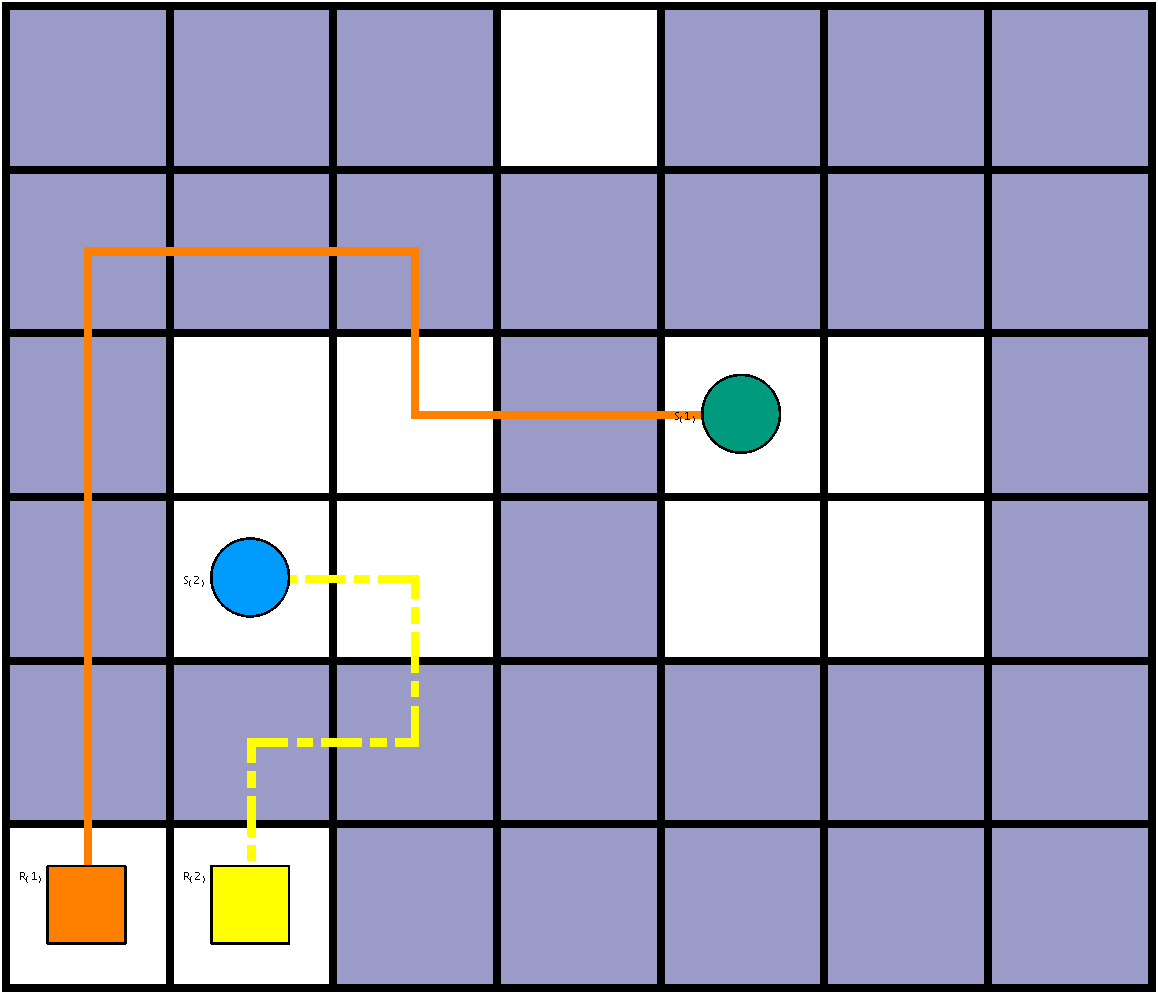
\includegraphics[scale=0.2]{img/asprilo_nc.png}
    \caption{Asprilo visualization for plan from Listing 16 without constraint.}
\end{subfigure}%
\hspace{10px}
\begin{subfigure}{.45\textwidth}
    \centering
    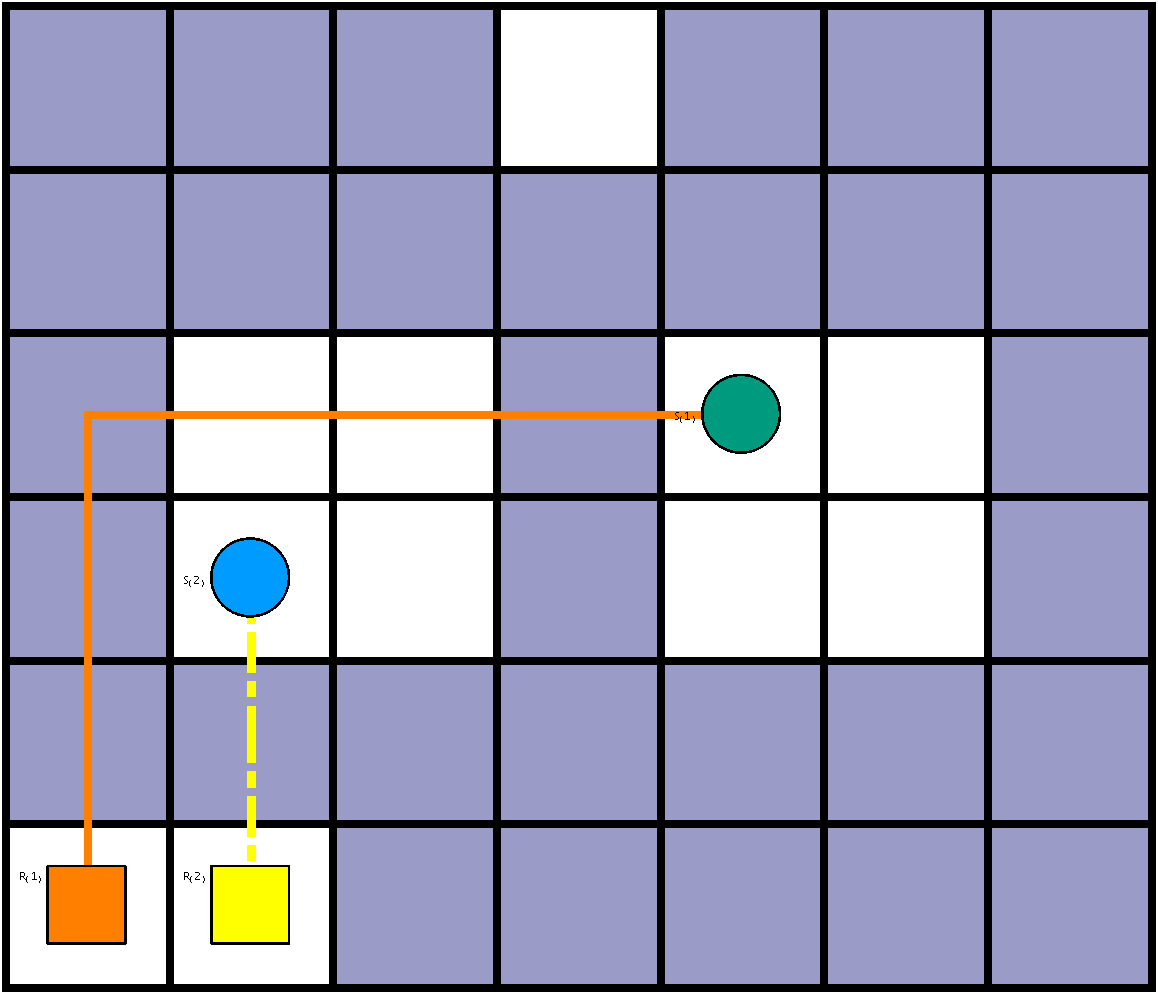
\includegraphics[scale=0.2]{img/asprilo_ur.png}
    \caption{Asprilo visualization for plan following constraint of Listing 17.}
\end{subfigure}
\caption{Images from $\asprilo$'s visualizer corresponding to presented plans. Robots are represented by squares and destinations by circles.}
\end{figure}


The constraint in Listing 17 removes any plan in which the temporal formula is not satisfied. In this case the formula corresponds to $\Next (\mathit{move(robot(R),UP)} \until (\mathit{move(robot(R),RIGHT)} \until \alwaysF \mathit{wait(robot(R))}))$, restricting plans to start with moves up followed by moves right and then waiting. The next operator $\Next$ is necessary at the beginning, since movements in $\asprilo$ start at time point 1. As we can notice, this constraint includes in its body the domain specific predicates \texttt{robot/1}, \texttt{right/1} and \texttt{up/1}.
To address the need of this predicates during the translation the instance is incorporated in the call to $\gringo$ as shown in the workflow overview\footnote{In this case we also require the inclusion of the initialization rules in Listing 14(1-9), as well as the auxiliary predicates for directions.}. 
Consequently, the call to the grounder instantiates the variables yielding one constraint for each robot. Then, the translation deals with the multiple constraints by generating several corresponding initial states of the automaton which are treated as independent automata. 


In the previous section we explained how the automata encoding assumes that all propositions included in the temporal/dynamic formula appear in predicate \texttt{in\_trace\_at/2} with their corresponding identifier from the reification process. 
Therefore, the plans generated by $\asprilo$, such as the one in Listing 15, need to be linked to the identifiers used in \texttt{in\_trace\_at/2}. To achieve such behavior, we construct the additional predicate \texttt{id\_map/2} during the translation of the automata. In this predicate, we gather the linearized abstract syntax tree from gringo into a tuple for a more readable mapping of identifiers. Using this predicate, we write the encoding, which we call `glue', linking all the domain-specific predicates used in the temporal constraint with \texttt{in\_trace\_at/2}. 

\begin{center}
    \begin{lstlisting}[] 
in_trace_at(I,T) :- 
    move(robot(R),(X,Y),T), 
    id_map(I,("move",("robot",N),(X,Y))).

in_trace_at(I,T) :- 
    wait(robot(R),(X,Y),T), 
    id_map(I,("wait",("robot",N))).
    \end{lstlisting}
\captionof{lstlisting}{Glue encoding for movement and position predicates in $\asprilo$.}
\end{center}

The `glue' encoding is then passed to the last call to $\clingo$ along with the instance and planning encoding. Even though the requirement of such an ad-hoc construction could be avoided by using an external script, we opted for an implementation using only ASP. Thus, this additional encoding must be included to complete the integration of any application to our approach.






\section{Experiments  }

\subsection{Setup}

For the experiments, we evaluated our implementation using different temporal constraints and initial states on the the simplified $\asprilo$ domain. The presented results ran using $\clingo$ 5.4.0 on an Intel Xeon E5-2650v4 under Debian GNU/Linux 9, with a memory of 20 GB and a timeout of 20 min per instance.

Throughout the experiments, we use three temporal constraints to limit the movements of robots. These constraints make use of additional predicates, which are included as part of the planning encoding. The first constraint is shown in Listing 19 and it restricts robots to move vertically before horizontally (allowing pauses between movements). Such constraint corresponds to the temporal formula $\neg\; \mathit{move\_horizontally(robot(R))} \until (\alwaysF \;\neg \;\mathit{move\_vertically(robot(R)))}$.

\begin{center}
    \begin{lstlisting}[] 
:- not &tel{(~ move_horizontally(robot(R)) ) >? 
                (>* ~ move_vertically(robot(R))) },
    robot(R).
    \end{lstlisting}
\captionof{lstlisting}{Move vertically before horizontally in $\LTLf$ .}
\end{center}

We can also express this constraint in $\LDLf$ using the equivalent formula \\ $\deventually{ (\mathit{no\_move\_horizontally(robot(R))} ; \top)^\ast} \dalways{\top^\ast} \mathit{no\_move\_vertically(robot(R))}$. \\The integration of predicates \texttt{no\_move\_horizontally/1} and \texttt{no\_move\_vertically/1} into the encoding is necessary to account for the aforementioned restrictions on this logic.

\begin{center}
    \begin{lstlisting}[] 
:- not &del{ *( ? no_move_horizontally(robot(R)) ;; &true ) .>? 
             ( (* &true ) .>* no_move_vertically(robot(R)) )}, 
    robot(R).
    \end{lstlisting}
\captionof{lstlisting}{Move vertically before horizontally in $\LDLf$ .}
\end{center}

The constraint to enforce horizontal movements before vertical ones is defined analogously to Listing 19 and Listing 20. For the last constraint, we ensure that robots move only in one direction in the x axis (right or left) and in one direction in the y axis (up or down). 

\begin{center}
    \begin{lstlisting}[] 
:- not &tel{ (>* (~ move_right(robot(R)))) |  
             (>* (~ move_left(robot(R)))) }, 
    robot(R).

:- not &tel{ (>* (~ move_up(robot(R)))) |  
             (>* (~ move_down(robot(R)))) }, 
    robot(R).
    \end{lstlisting}
\captionof{lstlisting}{Never both directions in $\LTLf$.}
\end{center}

By applying the equivalences for each operator we can translate the first formula in Listing 20 to one on $\LDLf$, namely $\deventually{(\dalways{\top^\ast}~move\_right(robot(R)))? + (\dalways{\top^\ast}~move\_left(robot(R)))?}\top$. This formula, however, does not follow our restrictions given that the test construct is applied to a formula with the box operator. Therefore, this constraint required some adjustments to be written under our specification, yielding the encoding in Listing 22.


\begin{center}
    \begin{lstlisting}[] 
:- not &del{ *(&true ;; ? no_move_right(robot(R))) +
             *(&true ;; ? no_move_left(robot(R))) .>?
             (&true.>* &false) }, 
    robot(R).

:- not &del{ *(&true ;; ? no_move_up(robot(R))) +
            *(&true ;; ? no_move_down(robot(R))) .>?
            (&true.>* &false) }, 
robot(R).
    \end{lstlisting}
\captionof{lstlisting}{Never both directions in $\LDLf$.}
\end{center}

Regarding the planning instances, we consider warehouses defined by configurations varying in size and number of robots. In the presented results, we follow the naming format for $\asprilo$ instances, where name \textit{xN\_yM\_rO} refers to instances of grid size $N\times M$ with $O$ robots.  
We also explored two different types of arrangements of the warehouse. A \emph{structured} one, where the robots are always in the lower left corner (Figure 4), as well as a second one, called \emph{grid} where robots are scattered in the space and obstacles can be present (Figure 5). 
For each configuration, we contemplate five initial states differing on the position of the destinations, represented by the last two numbers of the instance name.


\begin{figure}
    \centering
\begin{subfigure}{.45\textwidth}
    \centering
    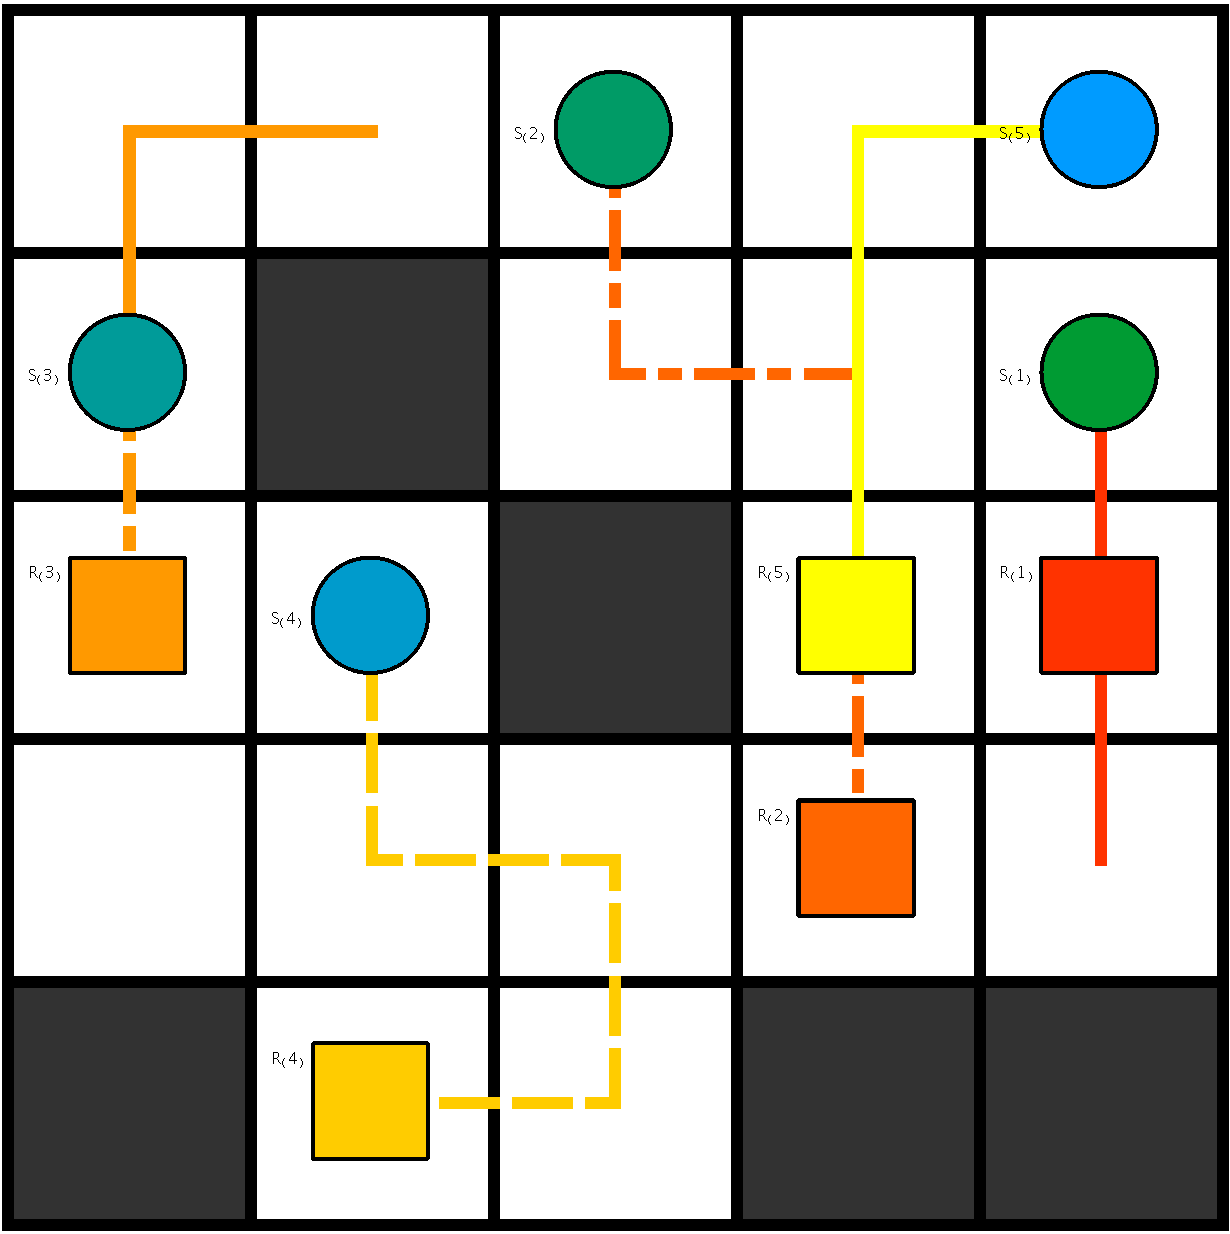
\includegraphics[scale=0.18]{img/g-asprilo-nc.png}
    \caption{Movement of robots without constraint.}
\end{subfigure}%
\hspace{10px}
\begin{subfigure}{.45\textwidth}
    \centering
    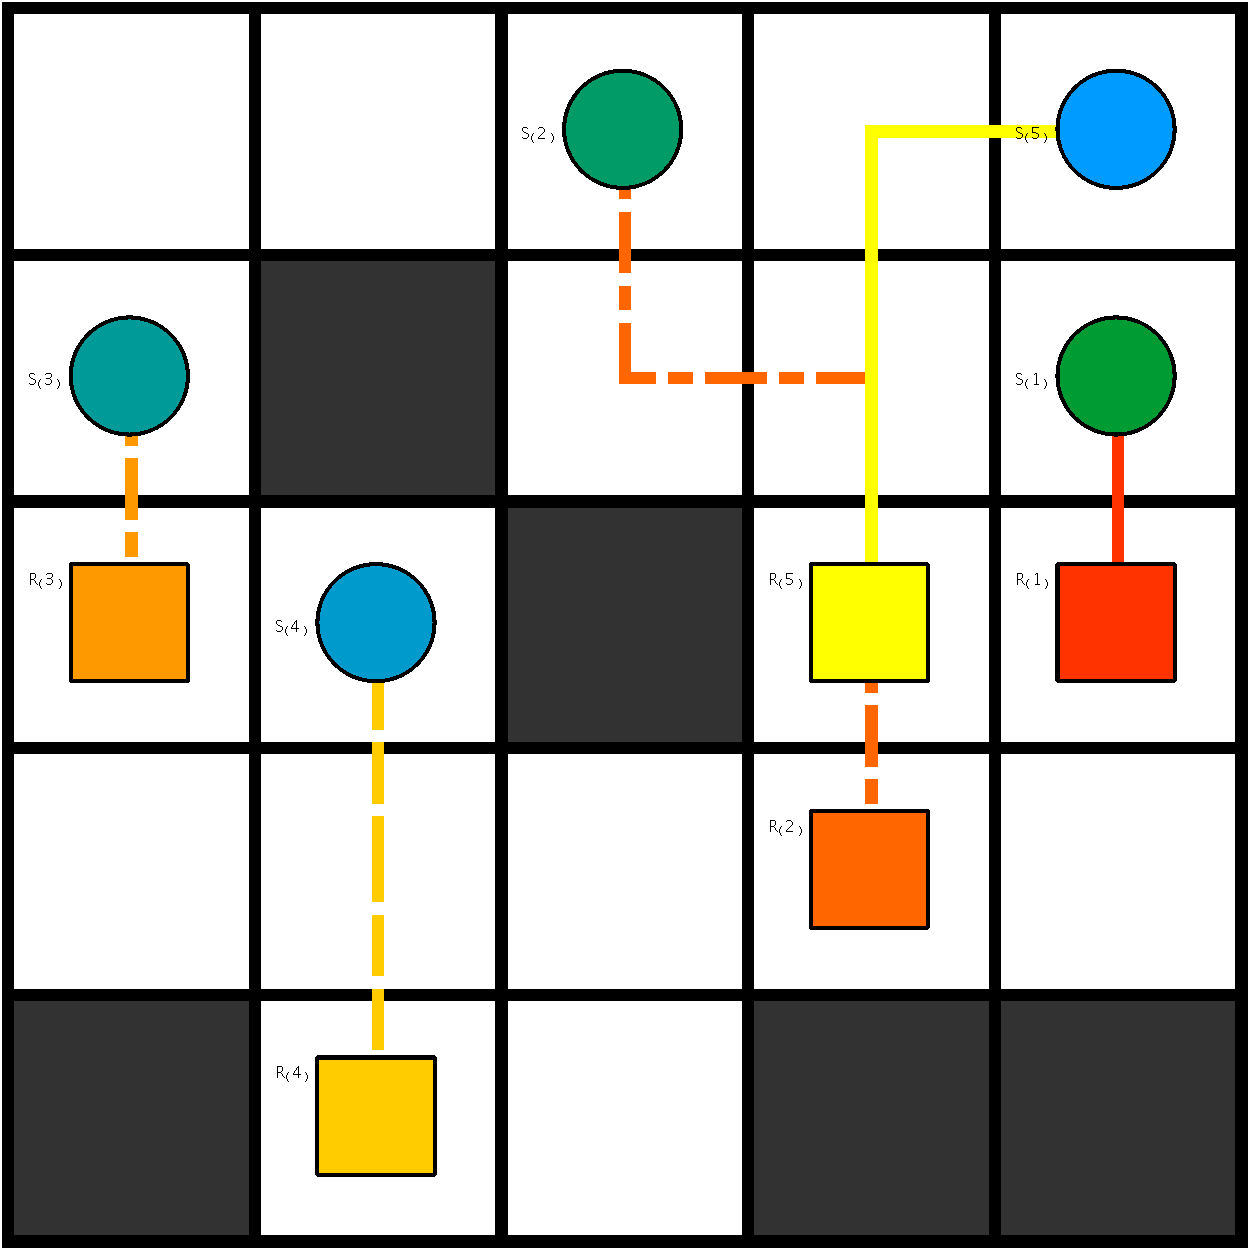
\includegraphics[scale=0.18]{img/g-asprilo.png}
    \caption{Applying constraint of never both directions.}
\end{subfigure}
\caption{Asprilo visualization for grid instance g-x5\_y5\_n20\_r5-05 with horizon 5, where cells in black represent obstacles.}
\end{figure}

\subsection{Results}


In the following results, we compare our implementation using automata from temporal and dynamic formulas against the encoding without these additional constraints, refereed to as `nc'. As baseline, we use a translation of the integrity constraints in $\LTLf$ to plain ASP trough $\TELf$, in the same way as in $\telingo$ \cite{cakamosc19a}. We use the name `asp' to refer to this last approach.

First, we present the most significant results encountered regarding the solving times of each method when searching for all the stable models of the program. In Figure 6, we can notice that, as expected, solving times are reduced drastically when applying a new integrity constraint to the program. In the case of no constraint, the solver reaches a timeout for all instances and constraints. Furthermore, the performance of the approach using $\LTLf$ is overall better than that for $\LDLf$. This behavior can be due to the different representation of states, either by numbers or predicates, between both methods. Moreover, it can be related to the differences of the translation of formulas. Overall, our baseline persist being considerably faster.



\begin{figure}[]
    \centering
    
    % This file was created by tikzplotlib v0.9.3.
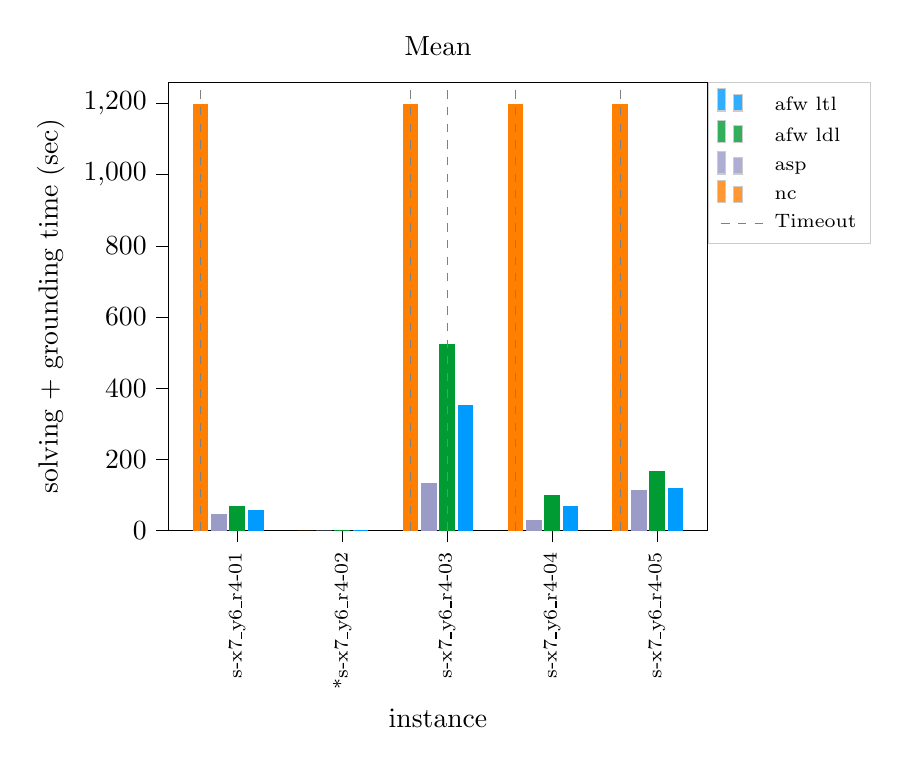
\begin{tikzpicture}

    \definecolor{color0}{rgb}{0,0.607843137254902,1}
    \definecolor{color1}{rgb}{0,0.607843137254902,0.2}
    \definecolor{color2}{rgb}{0.607843137254902,0.607843137254902,0.784313725490196}
    \definecolor{color3}{rgb}{1,0.498039215686275,0}
    
    \begin{axis}[
    legend cell align={left},
    legend style={font=\scriptsize,fill opacity=0.8, draw opacity=1, text opacity=1, at={(1,1)}, anchor=north west, draw=white!80!black},
    tick align=outside,
    tick pos=left,
    title={Mean},
    x grid style={white!69.0196078431373!black},
    xlabel={instance},
    xmin=-0.65875, xmax=4.48375,
    xtick style={color=black},
    xtick={0,1,2,3,4},
    xticklabel style = {font=\scriptsize,rotate=90.0},
    xticklabels={s-x7\_y6\_r4-01,*s-x7\_y6\_r4-02,s-x7\_y6\_r4-03,s-x7\_y6\_r4-04,s-x7\_y6\_r4-05},
    y grid style={white!69.0196078431373!black},
    ylabel={solving + grounding time (sec)},
    ymin=0, ymax=1260.01051025391,
    ytick style={color=black}
    ]
    \draw[draw=none,fill=color0] (axis cs:0.25,0) rectangle (axis cs:0.1,57.9530029296875);
    \addlegendimage{ybar,ybar legend,draw=none,fill=color0};
    \addlegendentry{afw ltl}
    
    \draw[draw=none,fill=color0] (axis cs:1.25,0) rectangle (axis cs:1.1,0.0643333345651627);
    \draw[draw=none,fill=color0] (axis cs:2.25,0) rectangle (axis cs:2.1,353.798980712891);
    \draw[draw=none,fill=color0] (axis cs:3.25,0) rectangle (axis cs:3.1,67.5556640625);
    \draw[draw=none,fill=color0] (axis cs:4.25,0) rectangle (axis cs:4.1,120.026000976562);
    \draw[draw=none,fill=color1] (axis cs:0.075,0) rectangle (axis cs:-0.075,68.9150009155273);
    \addlegendimage{ybar,ybar legend,draw=none,fill=color1};
    \addlegendentry{afw ldl}
    
    \draw[draw=none,fill=color1] (axis cs:1.075,0) rectangle (axis cs:0.925,0.0816666707396507);
    \draw[draw=none,fill=color1] (axis cs:2.075,0) rectangle (axis cs:1.925,524.588317871094);
    \draw[draw=none,fill=color1] (axis cs:3.075,0) rectangle (axis cs:2.925,98.8453369140625);
    \draw[draw=none,fill=color1] (axis cs:4.075,0) rectangle (axis cs:3.925,166.195343017578);
    \draw[draw=none,fill=color2] (axis cs:-0.1,0) rectangle (axis cs:-0.25,47.4580039978027);
    \addlegendimage{ybar,ybar legend,draw=none,fill=color2};
    \addlegendentry{asp}
    
    \draw[draw=none,fill=color2] (axis cs:0.9,0) rectangle (axis cs:0.75,0.0489999987185001);
    \draw[draw=none,fill=color2] (axis cs:1.9,0) rectangle (axis cs:1.75,132.566665649414);
    \draw[draw=none,fill=color2] (axis cs:2.9,0) rectangle (axis cs:2.75,30.5513324737549);
    \draw[draw=none,fill=color2] (axis cs:3.9,0) rectangle (axis cs:3.75,114.831665039062);
    \draw[draw=none,fill=color3] (axis cs:-0.275,0) rectangle (axis cs:-0.425,1199.98498535156);
    \addlegendimage{ybar,ybar legend,draw=none,fill=color3};
    \addlegendentry{nc}
    
    \draw[draw=none,fill=color3] (axis cs:0.725,0) rectangle (axis cs:0.575,0.0260000005364418);
    \draw[draw=none,fill=color3] (axis cs:1.725,0) rectangle (axis cs:1.575,1200.01000976562);
    \draw[draw=none,fill=color3] (axis cs:2.725,0) rectangle (axis cs:2.575,1200.0009765625);
    \draw[draw=none,fill=color3] (axis cs:3.725,0) rectangle (axis cs:3.575,1199.98596191406);
    \addplot [line width=0.28pt, white!50.1960784313725!black, dashed]
    table {%
    2 2.8421709430404e-14
    2 1260.01051025391
    };
    \addlegendentry{Timeout}
    \addplot [line width=0.28pt, white!50.1960784313725!black, dashed]
    table {%
    -0.35 2.8421709430404e-14
    -0.35 1260.01051025391
    };
    \addplot [line width=0.28pt, white!50.1960784313725!black, dashed]
    table {%
    1.65 2.8421709430404e-14
    1.65 1260.01051025391
    };
    \addplot [line width=0.28pt, white!50.1960784313725!black, dashed]
    table {%
    2.65 2.8421709430404e-14
    2.65 1260.01051025391
    };
    \addplot [line width=0.28pt, white!50.1960784313725!black, dashed]
    table {%
    3.65 2.8421709430404e-14
    3.65 1260.01051025391
    };
    \end{axis}
    
    \end{tikzpicture}
    
    \caption{Average of solving and grounding times for all three constraint with horizon 7 when obtaining all models in $\clingo$. Unsatisfiable instances are marked with *.}
\end{figure}

A higher horizon was required for bigger instances to become satisfiable, however, increasing the horizon led mostly to timeouts. Thus, we used clingo to compute only one model in order to examine more details about the programs for such larger instances. In Figure 7, we show the size of the program w.r.t. the number of rules and bodies with horizon 20. This figure presents instances grouping all initial states of each configuration. The proportion of rules and bodies remains proportional throughout the experiment, indicating that while programs increased in size of the new encoding, this was done by the same amount of rules as bodies. 
% Therefore, there was no special increase in facts.
We can also notice a minimal increase in size of the program when using the translation to ASP, whereas the introduction of the automata encoding almost doubles the original size.

\begin{figure}[]
    \centering
    
    % This file was created by tikzplotlib v0.9.3.
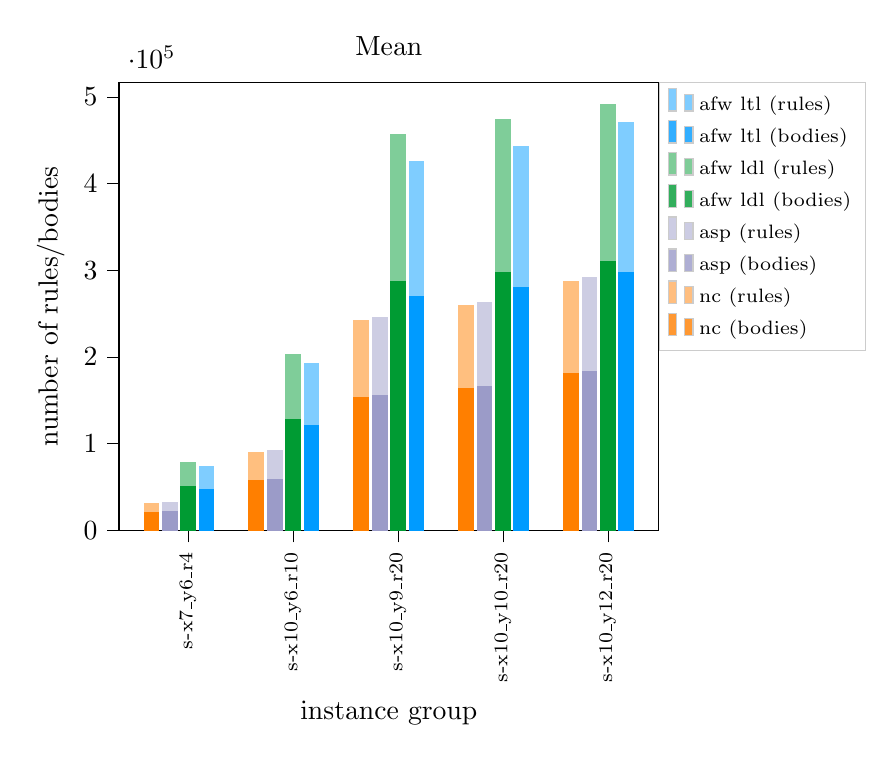
\begin{tikzpicture}

    \definecolor{color0}{rgb}{0,0.607843137254902,1}
    \definecolor{color1}{rgb}{0,0.607843137254902,0.2}
    \definecolor{color2}{rgb}{0.607843137254902,0.607843137254902,0.784313725490196}
    \definecolor{color3}{rgb}{1,0.498039215686275,0}
    
    \begin{axis}[
    legend cell align={left},
    legend style={font=\scriptsize,fill opacity=0.8, draw opacity=1, text opacity=1, at={(1,1)}, anchor=north west, draw=white!80!black},
    tick align=outside,
    tick pos=left,
    title={Mean},
    x grid style={white!69.0196078431373!black},
    xlabel={instance group},
    xmin=-0.65875, xmax=4.48375,
    xtick style={color=black},
    xtick={0,1,2,3,4},
    xticklabel style = {font=\scriptsize,rotate=90.0},
    xticklabels={s-x7\_y6\_r4,s-x10\_y6\_r10,s-x10\_y9\_r20,s-x10\_y10\_r20,s-x10\_y12\_r20},
    y grid style={white!69.0196078431373!black},
    ylabel={number of rules/bodies},
    ymin=0, ymax=516864.6,
    ytick style={color=black}
    ]
    \draw[draw=none,fill=color0,fill opacity=0.5] (axis cs:0.25,0) rectangle (axis cs:0.1,74920.3359375);
    \addlegendimage{ybar,ybar legend,draw=none,fill=color0,fill opacity=0.5};
    \addlegendentry{afw ltl (rules)}
    
    \draw[draw=none,fill=color0,fill opacity=0.5] (axis cs:1.25,0) rectangle (axis cs:1.1,192576);
    \draw[draw=none,fill=color0,fill opacity=0.5] (axis cs:2.25,0) rectangle (axis cs:2.1,426149.65625);
    \draw[draw=none,fill=color0,fill opacity=0.5] (axis cs:3.25,0) rectangle (axis cs:3.1,443255.65625);
    \draw[draw=none,fill=color0,fill opacity=0.5] (axis cs:4.25,0) rectangle (axis cs:4.1,471535.34375);
    \draw[draw=none,fill=color0] (axis cs:0.25,0) rectangle (axis cs:0.1,48106);
    \addlegendimage{ybar,ybar legend,draw=none,fill=color0};
    \addlegendentry{afw ltl (bodies)}
    
    \draw[draw=none,fill=color0] (axis cs:1.25,0) rectangle (axis cs:1.1,121728);
    \draw[draw=none,fill=color0] (axis cs:2.25,0) rectangle (axis cs:2.1,269848.34375);
    \draw[draw=none,fill=color0] (axis cs:3.25,0) rectangle (axis cs:3.1,280269);
    \draw[draw=none,fill=color0] (axis cs:4.25,0) rectangle (axis cs:4.1,297466.65625);
    \draw[draw=none,fill=color1,fill opacity=0.5] (axis cs:0.075,0) rectangle (axis cs:-0.075,79077);
    \addlegendimage{ybar,ybar legend,draw=none,fill=color1,fill opacity=0.5};
    \addlegendentry{afw ldl (rules)}
    
    \draw[draw=none,fill=color1,fill opacity=0.5] (axis cs:1.075,0) rectangle (axis cs:0.925,202942.671875);
    \draw[draw=none,fill=color1,fill opacity=0.5] (axis cs:2.075,0) rectangle (axis cs:1.925,456794);
    \draw[draw=none,fill=color1,fill opacity=0.5] (axis cs:3.075,0) rectangle (axis cs:2.925,473870);
    \draw[draw=none,fill=color1,fill opacity=0.5] (axis cs:4.075,0) rectangle (axis cs:3.925,492252);
    \draw[draw=none,fill=color1] (axis cs:0.075,0) rectangle (axis cs:-0.075,50756.66796875);
    \addlegendimage{ybar,ybar legend,draw=none,fill=color1};
    \addlegendentry{afw ldl (bodies)}
    
    \draw[draw=none,fill=color1] (axis cs:1.075,0) rectangle (axis cs:0.925,128354.6640625);
    \draw[draw=none,fill=color1] (axis cs:2.075,0) rectangle (axis cs:1.925,288035.34375);
    \draw[draw=none,fill=color1] (axis cs:3.075,0) rectangle (axis cs:2.925,298441.34375);
    \draw[draw=none,fill=color1] (axis cs:4.075,0) rectangle (axis cs:3.925,310720);
    \draw[draw=none,fill=color2,fill opacity=0.5] (axis cs:-0.1,0) rectangle (axis cs:-0.25,32725);
    \addlegendimage{ybar,ybar legend,draw=none,fill=color2,fill opacity=0.5};
    \addlegendentry{asp (rules)}
    
    \draw[draw=none,fill=color2,fill opacity=0.5] (axis cs:0.9,0) rectangle (axis cs:0.75,92716.3359375);
    \draw[draw=none,fill=color2,fill opacity=0.5] (axis cs:1.9,0) rectangle (axis cs:1.75,246315.328125);
    \draw[draw=none,fill=color2,fill opacity=0.5] (axis cs:2.9,0) rectangle (axis cs:2.75,263481.34375);
    \draw[draw=none,fill=color2,fill opacity=0.5] (axis cs:3.9,0) rectangle (axis cs:3.75,291792.34375);
    \draw[draw=none,fill=color2] (axis cs:-0.1,0) rectangle (axis cs:-0.25,22262.666015625);
    \addlegendimage{ybar,ybar legend,draw=none,fill=color2};
    \addlegendentry{asp (bodies)}
    
    \draw[draw=none,fill=color2] (axis cs:0.9,0) rectangle (axis cs:0.75,59867.33203125);
    \draw[draw=none,fill=color2] (axis cs:1.9,0) rectangle (axis cs:1.75,156003);
    \draw[draw=none,fill=color2] (axis cs:2.9,0) rectangle (axis cs:2.75,166453);
    \draw[draw=none,fill=color2] (axis cs:3.9,0) rectangle (axis cs:3.75,183666);
    \draw[draw=none,fill=color3,fill opacity=0.5] (axis cs:-0.275,0) rectangle (axis cs:-0.425,32003);
    \addlegendimage{ybar,ybar legend,draw=none,fill=color3,fill opacity=0.5};
    \addlegendentry{nc (rules)}
    
    \draw[draw=none,fill=color3,fill opacity=0.5] (axis cs:0.725,0) rectangle (axis cs:0.575,90911);
    \draw[draw=none,fill=color3,fill opacity=0.5] (axis cs:1.725,0) rectangle (axis cs:1.575,242698);
    \draw[draw=none,fill=color3,fill opacity=0.5] (axis cs:2.725,0) rectangle (axis cs:2.575,259864);
    \draw[draw=none,fill=color3,fill opacity=0.5] (axis cs:3.725,0) rectangle (axis cs:3.575,288175);
    \draw[draw=none,fill=color3] (axis cs:-0.275,0) rectangle (axis cs:-0.425,21771);
    \addlegendimage{ybar,ybar legend,draw=none,fill=color3};
    \addlegendentry{nc (bodies)}
    
    \draw[draw=none,fill=color3] (axis cs:0.725,0) rectangle (axis cs:0.575,58638);
    \draw[draw=none,fill=color3] (axis cs:1.725,0) rectangle (axis cs:1.575,153541);
    \draw[draw=none,fill=color3] (axis cs:2.725,0) rectangle (axis cs:2.575,163991);
    \draw[draw=none,fill=color3] (axis cs:3.725,0) rectangle (axis cs:3.575,181204);
    \end{axis}
    
    \end{tikzpicture}
    
    \caption{Average number of rules and bodies for all three constraint with horizon 20 when obtaining one model. Instances are grouped by configuration. }
\end{figure}


Next, we decided to inspect the scalability of the implementation for both temporal and dynamic logic. This was done by increasing the horizon and asking only for the first model. The results are shown in Figure 8 and show a similar behavior between both models. Interestingly, the solving time for the dynamic formulas is only better on the instances with the configuration of $10\times 10$ and 20 robots.


\begin{figure}[]
    \centering
    
    % This file was created by tikzplotlib v0.9.3.
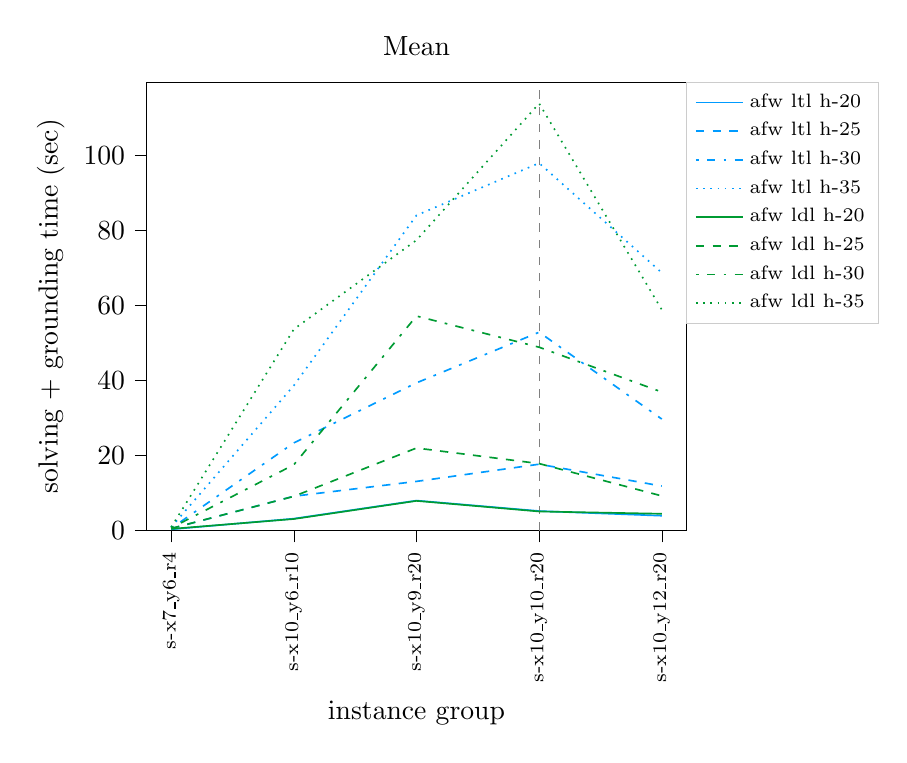
\begin{tikzpicture}

    \definecolor{color0}{rgb}{0,0.607843137254902,1}
    \definecolor{color1}{rgb}{0,0.607843137254902,0.2}
    
    \begin{axis}[
    legend cell align={left},
    legend style={font=\scriptsize,fill opacity=0.8, draw opacity=1, text opacity=1, at={(1,1)}, anchor=north west, draw=white!80!black},
    tick align=outside,
    tick pos=left,
    title={Mean},
    x grid style={white!69.0196078431373!black},
    xlabel={instance group},
    xmin=-0.2, xmax=4.2,
    xtick style={color=black},
    xtick={0,1,2,3,4},
    xticklabel style = {font=\scriptsize,rotate=90.0},
    xticklabels={s-x7\_y6\_r4,s-x10\_y6\_r10,s-x10\_y9\_r20,s-x10\_y10\_r20,s-x10\_y12\_r20},
    y grid style={white!69.0196078431373!black},
    ylabel={solving + grounding time (sec)},
    ymin=0, ymax=119.437843351066,
    ytick style={color=black}
    ]
    \addplot [semithick, color0, opacity=1]
    table {%
    0 0.327666670084
    1 3.15793347358704
    2 7.97200012207031
    3 5.18893337249756
    4 3.93733334541321
    };
    \addlegendentry{afw ltl h-20}
    \addplot [line width=0.28pt, white!50.1960784313725!black, dashed, forget plot]
    table {%
    3 3.5527136788005e-15
    3 119.437843351066
    };
    \addplot [semithick, color0, opacity=1, dashed]
    table {%
    0 0.508133351802826
    1 9.13133335113525
    2 13.082667350769
    3 17.6627330780029
    4 11.8399991989136
    };
    \addlegendentry{afw ltl h-25}
    \addplot [semithick, color0, opacity=1, dash pattern=on 1pt off 3pt on 3pt off 3pt]
    table {%
    0 0.570133328437805
    1 23.3456649780273
    2 39.3339996337891
    3 52.8310050964355
    4 29.6908664703369
    };
    \addlegendentry{afw ltl h-30}
    \addplot [semithick, color0, opacity=1, dotted]
    table {%
    0 0.892533302307129
    1 38.6154670715332
    2 83.9641952514648
    3 97.8827285766602
    4 68.6672668457031
    };
    \addlegendentry{afw ltl h-35}
    \addplot [semithick, color1, opacity=1]
    table {%
    0 0.427333325147629
    1 3.07173347473145
    2 7.8985333442688
    3 5.07393312454224
    4 4.45966672897339
    };
    \addlegendentry{afw ldl h-20}
    \addplot [semithick, color1, opacity=1, dashed]
    table {%
    0 0.549266636371613
    1 9.10186672210693
    2 21.9740009307861
    3 17.8249340057373
    4 9.21719932556152
    };
    \addlegendentry{afw ldl h-25}
    \addplot [semithick, color1, opacity=1, dash pattern=on 1pt off 3pt on 3pt off 3pt]
    table {%
    0 0.688400030136108
    1 17.520601272583
    2 57.1371955871582
    3 48.8288612365723
    4 36.8923301696777
    };
    \addlegendentry{afw ldl h-30}
    \addplot [semithick, color1, opacity=1, dotted]
    table {%
    0 0.884466648101807
    1 53.6264686584473
    2 77.3668670654297
    3 113.765930175781
    4 58.8269348144531
    };
    \addlegendentry{afw ldl h-35}
    \end{axis}
    
    \end{tikzpicture}
    
    \caption{Average solving times for all three constraint with horizons 20 to 35, when obtaining one model. Instances are grouped by configuration. }
\end{figure}


For our last analysis, we examined the number of choices and conflicts found by the solver for each approach. This was done for instances using the grid configuration. Results on Table 3 correspond to the number of conflicts when computing all models with a horizon of 5. 
Unlike the rest of the analysis, we here show the results only for the constraint ensuring robots do not move in both directions (listings 21 and 22). 
As we can observe in Table 3, the numbers decreased in over one order of magnitude for all satisfiable instances. 
Particularly, in the case of instance $g-x5\_y5\_n20\_r5-05$ (Figure 5), where 5 obstacles are presented\footnote{The number of obstacles is calculated based on the name as follows: $O=X\times Y-N$}, we can see a drastical improvement. Some of the presented instances become unsatisfied when including the constraints, due to the presence of obstacles which can only be avoided by moving in both directions. Furthermore, the number of conflicts is reduced in half when using temporal instead of dynamic logic.
A similar evaluation was performed for the number of choices in the program (Table 4). Here we recognize the same type of reduction. Although, in this case, the difference of choices between both logics is not as evident. As final remarks on these results, we notice an improvement on the use of the automata approach against our baseline for the first two instances. However, this gain is not encountered in the rest of the experiments.






\begin{table}
\centering
\begin{tabular}{|l|r|r|r|r|r|r|r|r|}
    \hline
    {} &  \textbf{afw ltl}&    \textbf{afw ldl} &    \textbf{asp} &    \textbf{nc}  \\
    \hline
    g-x5\_y5\_n20\_r5-01 &                        162 &                            340 &                        366 &                      7713 \\
    g-x5\_y5\_n20\_r5-02 &                         87 &                             64 &                        102 &                       218 \\
    g-x5\_y5\_n20\_r5-03 &                          1* &                              1* &                          1* &                         1* \\
    g-x5\_y5\_n20\_r5-04 &                       6511 &                          13428 &                       1348 &                    153447 \\
    g-x5\_y5\_n20\_r5-05 &                      13972 &                          62683 &                       5967 &                   6871918 \\
    \hline
    \hline
    g-x5\_y5\_n25\_r5-01 &                     115477 &                         242147 &                      62126 &                  11891485 \\
    g-x5\_y5\_n25\_r5-02 &                          1* &                              1* &                          1* &                         1* \\
    g-x5\_y5\_n25\_r5-03 &                     287504 &                         716067 &                     166992 &                  23184916 \\
    g-x5\_y5\_n25\_r5-04 &                         22* &                             25* &                         29* &                   3490969 \\
    g-x5\_y5\_n25\_r5-05 &                          1* &                              1* &                          1* &                         1* \\
    \bottomrule
    \end{tabular}
    
\caption{Number of conflicts with horizon 5 obtaining all models of instances in the grid configuration for constraint "never both directions". Results marked with * refer to unsatisfiable status. Instances in the first half of the table have 5 obstacle, whereas the ones in the bottom half have none.}
\end{table}


\begin{table}
\centering

    \begin{tabular}{|l|r|r|r|r|r|r|r|r|}
% \toprule
\hline
{} &  \textbf{afw ltl}&    \textbf{afw ldl} &    \textbf{asp} &    \textbf{nc}  \\
% \midrule
\hline

g-x5\_y5\_n20\_r5-01 &                     1367 &                         1548 &                      976 &                   17884 \\
g-x5\_y5\_n20\_r5-02 &                      292 &                          273 &                      212 &                    1240 \\
g-x5\_y5\_n20\_r5-03 &                        0* &                            0* &                        0* &                       0* \\
g-x5\_y5\_n20\_r5-04 &                    51338 &                        58250 &                     4189 &                 1065833 \\
g-x5\_y5\_n20\_r5-05 &                   109212 &                       157972 &                    17941 &                26319932 \\ 
\hline
\hline
g-x5\_y5\_n25\_r5-01 &                  1027511 &                      1154285 &                   290203 &                35869208 \\
g-x5\_y5\_n25\_r5-02 &                        0* &                            0* &                        0* &                       0* \\
g-x5\_y5\_n25\_r5-03 &                  1506971 &                      1935528 &                   319479 &               195544240 \\
g-x5\_y5\_n25\_r5-04 &                       39* &                           64* &                       82* &                14355800 \\
g-x5\_y5\_n25\_r5-05 &                        0* &                            0* &                        0* &                       0* \\
\hline
\end{tabular}

    \caption{Number of choices with horizon 5 obtaining all models of instances in the grid configuration for constraint "never both directions". Results marked with * refer to unsatisfiable status. Instances in the first half of the table have 5 obstacle, whereas the ones in the bottom half have none.}
\end{table}
\section{Discussion  }\label{sec:discussion}

In this thesis, we provided a way to constraint planning domains by means of temporal and dynamic formulas \footnote{The source code can be found in \url{https://github.com/susuhahnml/atlingo}}.
With ASP being one of the leading modeling languages to reason in this field, new strategies to include temporal formalisms have emerged in the past decade.
Current extensions build on the wellknown ASP system $\clingo$ to formalize temporal reasoning in the non-monotonic context based on equilibrium logic.
By limiting such reasoning to integrity constraints we were able to encode a translation of temporal and dynamic formulas from the monotonic formalisms $\LTLf$ and $\LDLf$ into $\AFW$, based on the work by Vardi and De Giacomo \cite{giavar15a}. 

While choosing Alternating Automata instead of Nondeterministic Automata reduces the number of states from exponential to linear in the size of the formula, it also introduces conceptualization challenges. First of all, alternating automata were originally defined in the infinite context, therefore literature for finite adaptations remains scarce.
% Furthermore, some implementation restrictions were overcomed by using an intermediate representation of the automaton, whereas other required carefully analysis and refinement.
Secondly, even though the connection between linear temporal logic and automata theory has been explored for almost 40 years \cite{varwol86a}, this is not the case for linear dynamic logic for which there is a restricted amount of existent research. 
Consequently, throughout this work we had to overcome several obstacles leading to multiple adjustments in the definitions for $\LDLf$. 
During this adaptation, we found the need for future remodeling of the equivalences between alternating automata and linear dynamic logic. 


Using the theory enhancing capabilities of clingo, we were able to extend the modeling language with these formalisms. Clingo's functionalities allowed us to keep the translation process as well as the automaton representation and computations solely declarative. 
However, by keeping all the implementation in ASP, we faced some limitations. 
We were not able to generate numeric identifiers for the subformulas and therefore had to construct more complex representation based on nested predicates. 
Moreover, the absence of an external program to transform the strings obtained from the reification into predicates caused the need for an additional encoding in order to link the application domain to our approach.

Unfortunately, our experiments didn't reveal clear positive results. 
Altogether, the direct translation into ASP was more efficient, concerning memory, speed and search, compared to the use of our automaton encoding. 
We also noticed a better performance when using $\LTLf$ instead of $\LDLf$. 
This outcome might be influenced by the implementation differences regarding the representation of states, as well as the complexity of the specific formulas and their corresponding automata.
Further inspection on the solving process, by analyzing choices and conflicts, showed a huge reduction in the search when the constrains were incorporated. 

We believe part of the unsatisfactory results could be attributed to the application chosen for the evaluation. 
In the reduced $\asprilo$ domain finding a valid plan is not as difficult as it is in other cases were multiple tasks and actions are considered. 
When the complexity rises, obtaining plans without constrains becomes harder and thus temporal constraints could help to lead the solver towards the solution. 

Since the presented work was only a first prototype towards the use of automata to handle temporal formulas in ASP, it opens the area for future research.
Upcoming work could include exploiting $\clingo$'s capabilities for enhanced theory-solving even further by constructing a propagator which will outsource model checking to an automaton. 
Moreover, integrating temporal constructs in ASP is still a promising endeavour with the potential to enrich the modeling language, thus facilitating new techniques to tackle diverse dynamic problems.

\pgfplotsset{compat=newest}

% \url{potassco.org}


\begin{appendices}

\section{\\Negation under $\DHT$ evaluated as $\LDL$}


  \begin{definition}[\DHT{} satisfaction]\label{def:dhtsat}
    %\comment{T: unify $\mathbb{N}$ with $\omega$}
    An \HT{} trace $\thandt $ \emph{satisfies} an dynamic formula $\varphi$ at time point $k \in \mathbb{N}$, written $\thandt ,k \models \varphi$, if the following conditions hold:
    \begin{enumerate}
      \item $\thandt ,k \models \top$ and  $\thandt ,k \not\models \bot$
      \item $\thandt ,k \models a$ if $a \in H(k)$ for any atom $a \in \PV$
      \item $\thandt , k \models \deventually{\rho} \varphi$
        if $\thandt ,i \models \varphi$ \\
        for some $i$ with $(k,i) \in \Rel{\rho}{\thandt }$
      \item \label{def:dhtsat.3} $\thandt , k \models \dalways{\rho} \varphi$
        if $\langle \
        H', T \rangle,i \models \varphi$ \\
        for all $i$ with $(k,i) \in \Rel{\rho}{\langle \
        H', T \rangle}$ and all $\
        H' \in \{ \
        H, T \}$
    \end{enumerate}
    where, for any \HT{} trace $\M$, $\Rel{\rho}{\M} \subseteq \mathbb{N}^2$ is a relation on pairs of time points inductively defined as follows.
    \begin{enumerate}[itemsep=5pt]
    \setcounter{enumi}{4}
    \item $\Rel{\top}{\M} \ \eqdef \ \{\ (i,i+1) \ \mid i \in \mathbb{N}\ \}$
    \item $\Rel{\varphi?}{\M}  \ \eqdef \ \{\ (i,i) \mid \M,i \models \varphi\ \}$
    \item $\Rel{\rho_1{+}\rho_2}{\M}  \ \eqdef \ \Rel{\rho_2}{\M} \cup \Rel{\rho_2}{\M}$
    \item
    \(
    \begin{array}[t]{@{}r@{\,}c@{\,}l@{\;}c@{\;}l}
    \Rel{\rho_1{\,;\,}\rho_2}{\M} & \eqdef & \{\ (i,j) & \mid & (i,k) \in \, \Rel{\rho_1}{\M} \ \text{and}\\
                            &        &           &      & (k,j) \in \, \Rel{\rho_2}{\M} \ \text{for some } k \ \}
    \end{array}
    \)
    \item $\Rel{\rho^*}{\M} \ \eqdef \ \bigcup_{n\geq 0} \Rel{\rho^*}{\M}_n$ \ where
    \[
    \!\!
    \begin{array}{l@{\,}c@{\,}l@{\,}c@{\,}l}
    \Rel{\rho^*}{\M}_0     & \eqdef & \{\ (i,i)         & \mid & i \in \mathbb{N}\ \}\\[5pt]
    \Rel{\rho^*}{\M}_{n+1} & \eqdef &\Rel{\rho^*}{\M}_n & \cup & \\
                           &        & \{\ (i,j)         & \mid & (i,k) \in \, \Rel{\rho}{\M}    \ \text{ and}\\
                           &        &                   &      & (k,j) \in \, \Rel{\rho^*}{\M}_n  \text{ for some } k \}
    \qed
    \end{array}
    \]
    \end{enumerate}
    \end{definition}

\begin{lemma}[Persistence $\DHT$ \cite{bocadisc18a}]
    For a dynamic formula $\varphi$, a HT-trace $\thandt  $ and $i\geq 0$.

    1. $\ttandt, i \models \varphi$ iff $\bm{T},i \models \varphi$ in $\LDL$
    
    2. $\thandt  , i \models \varphi$ implies $\ttandt, i \models \varphi$. \emph{(Persistence)}
\end{lemma}

\begin{lemma}[$\DHT$ and \LDL]
    For a dynamic formula $\varphi$, a HT-trace $\thandt  $ and $i\geq 0$, it holds that $\thandt  , i\models \neg \varphi$ in $\DHT$ iff $\bm{T},i \not \models \varphi$ in $\LDL$.

\textbf{\emph{Proof.}}\footnote{Note that negation is considered syntactic sugar for dynamic formulas. This is addressed in more detail in the following subsection.}.

$\Rightarrow$) $\thandt  , i\models \neg \varphi$ implies $\ttandt, i\models \neg \varphi$ based on Lemma 3.2. Which in turn implies $\bm{T},i \models \neg \varphi$ in $\LDL$ from Lemma 3.1. Using the semantics of $\LDL$ we get $\bm{T},i \not\models \varphi$ in $\LDL$.

$\Leftarrow$) $\bm{T},i \not\models \varphi$ in $\LDL$ implies $\ttandt, i \not\models \varphi$ based on Lemma 4.1. Using the contrapositive the persistence property in Lemma 3.2, then $\thandt  , i \not\models \varphi$. With the semantics for $\DHT$ \cite{bocadisc18a} we can conclude $\thandt  , i \models  \neg \varphi$.
\end{lemma}

The previous lemmas also hold for $\THT$ and $\LTL$ \cite{agcadipevi13a}, but we won't make them explicit since all formulas in $\THT$ can be encoded in $\DHT$, $\THT \subset \DHT$ \cite{bocadisc18a}.
\end{appendices}

\newpage
% \vspace*{\fill}

\vfill\noindent
\begin{center}
  \textbf{Declaration of originality}
\end{center}

I hereby certify that the thesis I am submitting is entirely my own original work except where otherwise indicated. I am aware of the University's regulations concerning plagiarism, including those regulations concerning disciplinary actions that may result from plagiarism. Any use of the works of any other author, in any form, is properly acknowledged at their point of use.

\begin{center}\bfseries{\textbf{\textit{\textcolor{darkblue}{Eigenständigkeitserklärung}}}}
\end{center}

    \textit{\textcolor{darkblue}{
        Hiermit bestätige ich, dass die von mir eingereichte Dissertation vollständig meine eigene Originalarbeit ist, sofern nicht anders angegeben. Mir sind die Vorschriften der Universität bezüglich Plagiaten bekannt, einschließlich der Vorschriften bezüglich disziplinarischer Maßnahmen, die sich aus einem Plagiat ergeben können. Jegliche Verwendung der Werke anderer Autoren, in welcher Form auch immer, wird an der Verwendungsstelle ordnungsgemäß anerkannt.
    }}


\vspace*{80px}
\noindent
\hfill%
\begin{tabular}[t]{c}
  \rule{15em}{0.4pt}\\ Signature/\textit{\textcolor{darkblue}{Unterschrift}}
\end{tabular}%
\hfill%
\begin{tabular}[t]{c}
  \rule{15em}{0.4pt}\\ Place/\textit{\textcolor{darkblue}{Ort}},\hspace{3px} Date/\textit{\textcolor{darkblue}{Datum}}
\end{tabular}%
\hfill\strut
\newpage


\printbibliography{}

\end{document}
